
\chapter{环之于模，恰如概形之于……}
\label{ch:rings-modules-schemes}

初学环的定义之时，你很快便被引向了\trModule{}：一个环映射 $R\to S$ 赋予 $S$ 一个 $R$-\trModule{}结构，理想与商也都是\trModule{}；而\trShortExactSequence{} $0\to I\to R\to R/I\to 0$ 则是「$\catMod{R}$ 构成一个\trAbelianCategory，且这是一个有用的观念」的第一份迹象。

对\trScheme{} $X$，与\trModule{}相当的东西并不是 $\OO_X$-\trModule{}的全体，而是其中一个性态良好的子集（一个\trSubcategory{}！）——\trQCSheaf{}，也称\trQCSheaf。


\section{\trQCSheaf}

给定一个 $A$-\trModule{} $M$，我们在 \S4.1.5 中定义了 $\Spec A$ 上的一个 $\OO$-\trModule{} $\widetilde{M}$——它在 $D(f)$ 上的\trSection{}就是 $M_f$。（如果你还没有做过 \S4.1.5 的那些练习，眼下正是补完的好时机。）这些便是我们关于\trQCSheaf{}的「局部模型」。正如\trScheme{}是靠「把环粘合起来」来定义的，一个\trScheme{}之上的\trQCSheaf{}也是靠「把那些环上的模粘合起来」得到的。

\textbf{6.1.1.}\ \emph{\trhDefinition{}：\trQCSheaf{}的\trCategory。}\quad 设 $X$ 是一个\trScheme。一个 $\OO_X$-\trModule{} $\scr{F}$ 称为一个\textbf{\trQCSheaf}（quasicoherent sheaf），若对每个\trAffine\trOpenSubset{} $\Spec A\subset X$，都有某个 $A$-\trModule{} $M$，使得 $\scr{F}|_{\Spec A}\cong\widetilde{M}$。我们取\trMorphism{}为「作为 $\OO_X$-\trModule{}的\trMorphism」，从而把概形 $X$ 上的诸\trQCSheaf{}做成一个\trCategory{} $\catQCo_X$。

\textbf{6.1.2.\ \trhTheorem。}\ ——\ \emph{设 $X$ 是一个\trScheme，$\scr{F}$ 是一个 $\OO_X$-\trModule。设 $P$ 是诸\trAffine\trOpenSubscheme{} $\Spec A\subset X$ 所享有的如下性质：存在某个 $A$-\trModule{} $M$，使得 $\scr{F}|_{\Spec A}\cong\widetilde{M}$。则 $P$ 满足\trAffineCommunicationLemma{}~5.3.2 的两条假设。}

于是，要检验一个 $\OO$-\trModule{}的\trQC{}性，只需在覆盖 $X$ 的一族仿射开集上加以检验即可。例如，$\widetilde{M}$ 就是 $\Spec A$ 上的一个\trQCSheaf。\cref{ex:module-maps-sheaf-maps}表明，$\catMod{A}$ 与 $\catQCo_{\Spec A}$ 这两个\trCategory{}本质上相同（我们已经描述了一个等价 $\catMod{A}\;\tilde{\longleftrightarrow}\;\catQCo_{\Spec A}$）。

\emph{证明。}\ 照例，\trAffineCommunicationLemma{}~5.3.2 的第一条假设更容易：若 $\Spec A$ 具有性质 $P$，则\trDistinguishedOpen{} $\Spec A_f$ 亦然：若 $M$ 是一个 $A$-\trModule，则作为 $\OO_{\Spec A_f}$-\trModule{}的层，有 $\widetilde{M}|_{\Spec A_f}\cong\widetilde{M_f}$（两边在诸\trDistinguishedOpen{}及其\trRestrictionMap{}的层面上一致）。

接下来我们证明\trAffineCommunicationLemma{}~5.3.2 的第二条假设。设已给定：
\begin{itemize}
\item 一个 $\OO_{\Spec A}$-\trModule{} $\scr{F}$；
\item 生成 $A$ 的诸元素 $f_1,\dots,f_n$；
\item 一些 $A_{f_i}$-\trModule{} $M_i$；以及
\item 一些\trIsomorphism{} $\phi_i\colon\scr{F}|_{D(f_i)}\tilde{\longrightarrow}\widetilde{M}_i$。
\end{itemize}
这些\trIsomorphism
\[
\begin{tikzcd}[row sep=2.4em, column sep=3.2em]
 & \scr{F}|_{D(f_i)\cap D(f_j)} \ar[dl,"\sim"] \ar[dr,"\sim"] \\
\widetilde{M}_i|_{D(f_i)\cap D(f_j)} & & \widetilde{M}_j|_{D(f_i)\cap D(f_j)}
\end{tikzcd}
\]
（通过在 $D(f_i)\cap D(f_j)$ 上取\trSection）给出 $A_{f_if_j}$-\trModule{}的一些\trIsomorphism{} $\phi_{ij}\colon(M_i)_{f_j}\tilde{\longrightarrow}(M_j)_{f_i}$，它们满足\trCocycleCondition{} \eqref{eq:cocycle-condition}。作为一种富有暗示性的记号，令 $M_{ij}:=(M_i)_{f_j}$（借助 $\phi_{ij}$ 把它与 $(M_j)_{f_i}$ 等同）。

我们寻找一个 $A$-\trModule{} $M$，使之带有\trIsomorphism{} $\widetilde{M}\;\tilde{\longleftrightarrow}\;\scr{F}$；而 \eqref{eq:module-equalizer-sequence} 提示我们应当如下定义 $M$：
\begin{equation*}\tag{6.1.2.1}\label{eq:m-equalizer-definition}
0\longrightarrow M\longrightarrow M_1\times\cdots\times M_n\overset{\gamma}{\longrightarrow}M_{12}\times M_{13}\times\cdots\times M_{(n-1)n}.
\end{equation*}
（\eqref{eq:module-equalizer-sequence} 处的讨论提示了映射 $\gamma$ 该怎样定义，需配上恰当的正负号。）翻译过来就是：$M=\ker(\gamma)$。若我们能在每个 $D(f_i)$ 上描述一个\trIsomorphism{} $\widetilde{M}|_{D(f_i)}\tilde{\longrightarrow}\widetilde{M}_i$（等价地，$A_{f_i}$-\trModule{}的一个\trIsomorphism{} $M_{f_i}\tilde{\longrightarrow}M_i$），使得 $\Spec A_{f_if_j}$ 上诸\trSheaf{}的三角形
\[
\begin{tikzcd}[row sep=2.4em, column sep=3.2em]
 & \widetilde{M}|_{D(f_i)\cap D(f_j)} \ar[dl,"\sim"] \ar[dr,"\sim"] \\
\widetilde{M}_i|_{D(f_i)\cap D(f_j)} \ar[rr,"\widetilde{\phi}_{ij}"',"\sim"] & & \widetilde{M}_j|_{D(f_i)\cap D(f_j)}
\end{tikzcd}
\]
交换（对一切 $i$, $j$），那么\cref{ex:gluing-sheaves-cocycle}（关于粘合\trSheaf{}的那条练习）便给出我们想要的\trIsomorphism{} $\widetilde{M}\;\tilde{\longleftrightarrow}\;\scr{F}$。

由\cref{ex:module-maps-sheaf-maps}，我们只需描述一个\trIsomorphism{} $M_{f_i}\tilde{\longrightarrow}M_i$，使得诸三角形
\begin{equation*}\tag{6.1.2.2}\label{eq:triangle-modules-fi-fj}
\begin{tikzcd}[row sep=2.4em, column sep=3.2em]
 & M_{f_if_j} \ar[dl,"\sim"] \ar[dr,"\sim"] \\
(M_i)_{f_j} \ar[rr,"\phi_{ij}"] & & (M_j)_{f_i}
\end{tikzcd}
\end{equation*}
交换。

为记号方便起见，不妨设 $i=1$。由于\trLocalization{}是\trExact{}的，从 \eqref{eq:m-equalizer-definition} 可得正合列
\[
0\longrightarrow M_{f_1}\longrightarrow(M_1)_{f_1}\times\cdots\times(M_n)_{f_1}\overset{\gamma_{f_1}}{\longrightarrow}(M_{12})_{f_1}\times(M_{13})_{f_1}\times\cdots\times(M_{(n-1)n})_{f_1}.
\]
我们将证明
\begin{equation*}\tag{6.1.2.3}\label{eq:m1-exact-beta-gamma}
0\longrightarrow M_1\overset{\beta}{\longrightarrow}(M_1)_{f_1}\times\cdots\times(M_n)_{f_1}\overset{\gamma_{f_1}}{\longrightarrow}(M_{12})_{f_1}\times(M_{13})_{f_1}\times\cdots\times(M_{(n-1)n})_{f_1}
\end{equation*}
是正合的（你看出 $\beta$ 该怎样定义了吗？），由此便给出我们想要的\trIsomorphism{} $M_{f_1}\tilde{\longrightarrow}M_1$。我们把 \eqref{eq:m1-exact-beta-gamma} 改写为
\begin{equation*}\tag{6.1.2.4}\label{eq:m1-rewritten-alpha}
\begin{aligned}
0\longrightarrow M_1\longrightarrow{} &(M_1)_{f_1}\times(M_1)_{f_2}\times\cdots\times(M_1)_{f_n}\\
\overset{\alpha}{\longrightarrow}{} &(M_1)_{f_1f_2}\times\cdots\times(M_1)_{f_1f_n}\times(M_1)_{f_2f_3}\times\cdots\times(M_1)_{f_{n-1}f_n}.
\end{aligned}
\end{equation*}
但这恰恰就是正合列 \eqref{eq:module-equalizer-sequence}，只不过把环 $A$ 换成了 $A_{f_1}$，把\trModule{} $M$ 换成了 $M_1$。

\textbf{6.1.A.（练习）}\quad 把最后一根松线拴紧：为什么三角形 \eqref{eq:triangle-modules-fi-fj} 交换？\hfill$\square$

\extrahard\ \emph{行家注记：}\ 定理~6.1.2 的证明若表述得稍稍更谨慎一些，便表明\trQCSheaf{}满足\trFaithfullyFlat{}下降（faithfully flat descent）。

\textbf{6.1.3.\ 零星收尾话题。}

\textbf{6.1.B.\ 不重要的练习（并非每个 $\OO_X$-\trModule{}都是\trQCSheaf）。}\quad

(a)~设 $X=\Spec k[t]$。设 $\scr{F}$ 是支撑在原点 $[(t)]$ 处的\trSkyscraperSheaf，其群为 $k(t)$，并带有通常的 $k[t]$-\trModule{}结构。证明：这是一个 $\OO_X$-\trModule，但不是\trQCSheaf。（更一般地，若 $X$ 是一个\trIntegral\trScheme，而 $p\in X$ 不是\trGenericPoint，我们可以取在 $p$ 处支撑的\trSkyscraperSheaf，其群取为 $X$ 的\trFunctionField。除非在犯傻的情形下，这个\trSheaf{}不会是\trQC{}的。）更多的「是 $\OO_X$-\trModule{}却不是\trQCSheaf」的（病态）例子，参看练习~9.1.G 与 6.2.H。

(b)~设 $X=\Spec k[t]$。设 $\scr{F}$ 是支撑在\trGenericPoint{} $[(0)]$ 处的\trSkyscraperSheaf，其群为 $k(t)$。请赋予它一个 $\OO_X$-\trModule{}的结构。证明：它\emph{确实}是\trQCSheaf。描述 $X$ 的\trDistinguishedTopology{}（distinguished topology）中全部的\trRestrictionMap。（评注：你的论证在更一般的情形也适用，例如：当 $X$ 是一个带\trGenericPoint{} $\eta$ 的\trIntegral\trScheme，而 $\scr{F}$ 是摩天楼层 $i_{\eta,*}K(X)$ 时。）

\textbf{6.1.4.\ 无挠层（一条\trStalkLocal{}条件）与挠层。}\quad 称一个 $A$-\trModule{} $M$ 为\textbf{\trTorsionFree}（torsion-free）的，若 $a\mathrm{m}=0$ 蕴涵：要么 $a$ 是 $A$ 中的\trZerodivisor，要么 $\mathrm{m}=0$。

在 $A$ 是\trIntegralDomain{}的情形——这基本上是我们将要使用这一概念的唯一场合——\trTorsionFree{}性的定义可以改述为：$a\mathrm{m}=0$ 仅当 $a=0$ 或 $\mathrm{m}=0$ 时成立。此时，$M$ 的\textbf{\trTorsionSubmodule{}}（torsion submodule）记作 $M_{\mathrm{tors}}$，由 $M$ 中被 $A$ 的某个非零元素零化的那些元素组成。（若 $A$ 不是\trIntegralDomain，这一构造未必给出一个 $A$-\trModule。）显然，$M$ 是\trTorsionFree{}的当且仅当 $M_{\mathrm{tors}}=0$。我们称\trIntegralDomain{} $A$ 上的一个\trModule{} $M$ 为\textbf{挠}（torsion）的，若 $M=M_{\mathrm{tors}}$；这等价于 $M\otimes_A K(A)=0$。

若 $X$ 是一个\trScheme，则一个 $\OO_X$-\trModule{} $\scr{F}$ 称为\textbf{\trTorsionFree}的，若对一切 $\mathfrak{p}$，$\scr{F}_\mathfrak{p}$ 都是\trTorsionFree{}的 $\OO_{X,\mathfrak{p}}$-\trModule。

\textbf{6.1.5.}\ \emph{\trhDefinition{}：既约概形上的挠拟凝聚层。}\quad 受上面对 $M_{\mathrm{tors}}$ 的定义的启发，我们称\emph{既约}概形上的一个\trQCSheaf{}是\textbf{挠}的，若它在每个\trIrreducibleComponent{}的\trGenericPoint{}处的\trStalk{}为 $0$。我们主要将把它用于\trRegular\trCurve{}上的诸\trCoherentSheaf——在那里这个概念的确十分简单（见练习~14.3.F(b)）——但在文献中，它也会在更一般的情形下出现。


\section{用\trDistinguishedAffineBase{}刻画\trQC{}性}

因为\trQCSheaf{}在局部上都呈一种十分特殊的形态，要想「认识」一个\trQCSheaf，我们只需知道诸\trSection{}在每个\trAffine\trOpenSet{}上是什么，以及如何把\trSection{}从一个\trAffine\trOpenSet{} $\mathscr{U}$ 限制到 $\mathscr{U}$ 的特异\trAffine\trOpenSubset{}上。我们将通过定义扎里斯基\trTopology{}的所谓\textbf{\trDistinguishedAffineBase{}}（distinguished affine base）来把这件事讲精确——它并非通常意义下的\trBase。这是对「\trSheafOnBase」观念的一种精细化。这一番讨论的要点在于给出\trQC{}性的一个有用刻画，不过你或许愿意径直跳到 \S6.2.3。

\trDistinguishedAffineBase{}中的\trOpenSet，就是 $X$ 的诸\trAffine\trOpenSubset。我们已经观察到它们构成一个\trBase。但请把这一事实忘掉。我们喜爱的是诸\trDistinguishedOpen{} $\Spec A_f\hookrightarrow\Spec A$；至于随便哪个\trAffine\trOpenSubset{}开嵌入另一个之中的那种\trOpenEmbedding，我们并无真正的理解。所以我们干脆只记住那些「好」的\trInclusionMap。

\textbf{6.2.1. \trhDefinition{}。}\quad 概形 $X$ 的\textbf{\trDistinguishedAffineBase{}}，就是「诸\trAffine\trOpenSet{}与诸特异\trInclusionMap」这份数据。

换言之，我们只记住\trOpenSet{}中的一部分（诸\trAffine\trOpenSet），而且\emph{只记住它们之间的一部分\trMorphism}（诸特异\trMorphism）。给行家的：若你把一个\trTopology{}想成一个\trCategory{}（即\trOpenSet{}的\trCategory），那么我们所描述的便是一个\trSubcategory。

我们可以按显而易见的方式定义\trDistinguishedAffineBase{}上的\trSheaf{}：给每个\trAffine\trOpenSet{}配一个\trSet{}（或\trAbelianGroups、或\trRing），并且我们知道如何限制到诸\trDistinguishedOpen{}上。（\trIdentityAxiom{}与\trGluability{}公理的陈述，你应当自行想通。）

给定 $X$ 上的一个\trSheaf{} $\mathscr{F}$，我们便得到\trDistinguishedAffineBase{}上的一个\trSheaf。你能猜到我们正往哪里去：我们将证明，\trSheaf{}的全部信息都蕴含于\trDistinguishedAffineBase{}上的\trSheaf{}的信息之中。

作为热身，我们可以如下地复原诸\trStalk{}。（我们将隐含地只用到下面这个事实。设有\trOpenSubset{}组成的一个族，以及这些子集之间的\emph{某些}\trInclusionMap，使得对任取的一点 $p\in\mathscr{U}\cap\mathscr{V}$（$\mathscr{U}$、$\mathscr{V}$ 都属于我们的\trOpenSubset{}族），总存在某个 $\mathscr{W}$ 包含 $p$ 且含于 $\mathscr{U}$ 与 $\mathscr{V}$ 之内，而 $\mathscr{W}\hookrightarrow\mathscr{U}$ 与 $\mathscr{W}\hookrightarrow\mathscr{V}$ 都属于我们的\trInclusionMap{}之族。在我们此处考虑的情形，这正是关键的命题~5.3.1：给定 $X$ 中任意两个\trAffine\trOpenSet{} $\Spec A$、$\Spec B$，$\Spec A\cap\Spec B$ 能够被一族「在 $\Spec A$ 与 $\Spec B$ 中同时特异」的\trAffine\trOpenSet{}覆盖。用华丽的语言说：由\trAffine\trOpenSet{}与特异\trInclusionMap{}组成的\trCategory{}构成一个\trFiltered{}集。）

\trStalk{} $\mathscr{F}_p$ 是\trColimit{} $\colim(f\in\mathscr{F}(\mathscr{U}))$，该\trColimit{}取遍所有含 $p$ 的\trOpenSet。我们把它与 $\colim(f\in\mathscr{F}(\mathscr{U}))$ 相比较，这里该\trColimit{}取遍所有含 $p$ 的\trAffine\trOpenSet{}与所有特异\trInclusionMap。你可以检验：其中一方的元素与另一方的元素相互对应。（仔细想想这件事！）

\textbf{6.2.A.（练习）}\quad 证明：\trDistinguishedAffineBase{}上一个\trSheaf{}的\trSection{}由该\trSection{}的诸\trGerm{}确定。

\textbf{6.2.2.\ \trhTheorem{}。}\ ——\
\begin{enumerate}[label=(\alph*)]
  \item \emph{\trDistinguishedAffineBase{}上的\trSheaf{} $\mathscr{F}^{\flat}$ 确定一个\trSheaf{} $\mathscr{F}$：它在相差唯一\trIsomorphism{}的意义下唯一，且限制到仿射基底上时即为 $\mathscr{F}^{\flat}$。（因此，若你从一个\trSheaf{}出发，取其在\trDistinguishedAffineBase{}上的\trSheaf，再取由此诱导的\trSheaf，你得到的正是出发时的那个\trSheaf。）}
  \item \emph{\trDistinguishedAffineBase{}上的\trSheaf{}之间的\trMorphism，唯一地确定诸\trSheaf{}之间的\trMorphism。}
  \item \emph{「\trDistinguishedAffineBase{}上」的 $\OO_X$-\trModule{}给出一个 $\OO_X$-\trModule。}
\end{enumerate}

这个证明与我们在 \S2.5 中那个「诸\trSheaf{}（在本质上）就是\trBase{}上的诸\trSheaf」的论证一模一样，用的也是「\trCompatibleGerm\trSheaf」这一构造。之所以不厌其烦地再讲一遍，主要是想让你亲眼看到：这里所需要的一切，无非是诸\trOpenSet{}构成一个\trFiltered{}集（或者在当前情形下，由\trOpenSet{}与特异\trInclusionMap{}构成的\trCategory{}是\trFiltered{}的）。

给行家的：(a) 与 (b) 所描述的，是「$X$ 的\trZariskiTopology{}上的诸\trSheaf」与「$X$ 的\trDistinguishedAffineBase{}上的诸\trSheaf」之间的一个\trEquivalenceOfCategories。

\emph{证明。}\ (a)~设 $\mathscr{F}^{\flat}$ 是\trDistinguishedAffineBase{}上的一个\trSheaf。那么我们可以定义诸\trStalk。

对 $X$ 的\emph{任何}\trOpenSet{} $\mathscr{U}$，定义\trCompatibleGerm\trSheaf
\[
\mathscr{F}(\mathscr{U}):=\Bigl\{(f_p\in\mathscr{F}^{\flat}_p)_{p\in\mathscr{U}}:\ \begin{array}{l}
\text{对一切 }p\in\mathscr{U}\text{，存在 }\mathscr{U}_p\text{ 使 }p\in\mathscr{U}_p\subset\mathscr{U}\text{，}\\
\text{且存在 }s\in\mathscr{F}^{\flat}(\mathscr{U}_p)\text{，使得对一切 }q\in\mathscr{U}_p\text{ 都有 }s_q=f_q
\end{array}\Bigr\},
\]
其中每个 $\mathscr{U}_p$ 都在我们的\trBase{}中，而 $s_q$ 指「$s$ 在 $q$ 处的\trGerm{}」。（照例，想为空集操心的人自便。）

这确实是一个\trSheaf{}：请说服自己，\trRestrictionMap、\trIdentityAxiom{}与\trGluability{}我们都已具备，而且来得相当轻易。

我接下来断言：若 $\mathscr{U}$ 在我们的\trBase{}中，则 $\mathscr{F}(\mathscr{U})=\mathscr{F}^{\flat}(\mathscr{U})$。我们显然有一个映射 $\mathscr{F}^{\flat}(\mathscr{U})\to\mathscr{F}(\mathscr{U})$。它在诸\trStalk{}上是\trIsomorphism，故由\cref{ex:isomorphisms-determined-by-stalks}，它是\trIsomorphism。

\textbf{6.2.B.（练习）}\quad 证明 (b)（对照\cref{ex:sheaf-morphisms-on-base}）。

\textbf{6.2.C.（练习）}\quad 证明 (c)（对照\cref{thm:ox-modules-on-base}）。

至此，定理~6.2.2 的证明便告完成。\hfill$\square$

\textbf{6.2.3. 用特异\trInclusionMap{}刻画\trQCSheaf。}\quad 我们将用这一视角，在诸 $\OO_X$-\trModule{}之中给出\trQCSheaf{}的一个有用刻画。设 $\mathscr{F}$ 是一个 $\OO_X$-\trModule，并设 $\Spec A_f\hookrightarrow\Spec A\subset X$ 是 $X$ 的一个\trAffine\trOpenSubscheme{}的\trDistinguishedOpen\trSubscheme。设 $\phi\colon\Gamma(\Spec A,\mathscr{F})\to\Gamma(\Spec A_f,\mathscr{F})$ 是\trRestrictionMap。$\phi$ 的源是一个 $A$-\trModule，目标是 $A_f$-\trModule，故由\trLocalization{}的\trUniversalProperty{}（\cref{ex:rings-localization-universal-property}），$\phi$ 自然地分解为：
\[
\begin{tikzcd}[row sep=2.6em, column sep=5.5em]
\Gamma(\Spec A,\mathscr{F}) \ar[rr,"\phi"] \ar[dr,"\otimes_A A_f"'] && \Gamma(\Spec A_f,\mathscr{F}) \\
& \Gamma(\Spec A,\mathscr{F})_f \ar[ur,"\alpha"] &
\end{tikzcd}
\]

\textbf{6.2.D.（十分重要的练习）}\quad 证明：一个 $\OO_X$-\trModule{} $\mathscr{F}$ 是\trQC{}的，当且仅当对每个这样的特异包含 $\Spec A_f\hookrightarrow\Spec A$，$\alpha$ 都是\trIsomorphism。

于是，一个\trQCSheaf{}（等价地）就是这样的数据：对每个\trAffine\trOpenSubset{}配有一个\trModule{}（即相应\trRing{}上的一个\trModule），使得\trDistinguishedOpen{} $\Spec A_f$ 上的那个\trModule，由对 $\Spec A$ 上的\trModule{}作\trLocalization{}而给出。

\textbf{6.2.E.（好练手：幂零层）}\quad 设 $A$ 是一个\trRing，$f\in A$。证明 $\mathfrak{N}(A_f)\cong\mathfrak{N}(A)_f$。用这件事在任意概形 $X$ 上定义／构造\trQC{}的\textbf{\trNilpotent\trSheaf}（sheaf of nilpotents）。这是（$\OO_X$ 的）\trIdeal\trSheaf{}的一个例子。

\textbf{6.2.4.}\ \emph{\trTensorProduct。}\quad $X$ 上\trQCSheaf{}范畴中的\trTensorProduct，也能借助\trAffine\trOpenSet{}得到一个干净的描述。

\textbf{6.2.F.（练习）}\quad 设 $\mathscr{F}$ 与 $\mathscr{G}$ 是概形 $X$ 上的两个\trQCSheaf。证明 $\mathscr{F}\otimes\mathscr{G}$ 是一个\trQCSheaf，并可由下述信息描述：若 $\Spec A\subset X$ 是一个\trAffine\trOpenSubset，且 $\Gamma(\Spec A,\mathscr{F})=M$、$\Gamma(\Spec A,\mathscr{G})=N$，则 $\Gamma(\Spec A,\mathscr{F}\otimes\mathscr{G})=M\otimes_A N$，而且\trRestrictionMap{} $\Gamma(\Spec A,\mathscr{F}\otimes\mathscr{G})\to\Gamma(\Spec A_f,\mathscr{F}\otimes\mathscr{G})$ 恰是\trLocalization{}映射 $M\otimes_A N\to(M\otimes_A N)_f\cong M_f\otimes_{A_f}N_f$。（我们用到了代数事实 $(M\otimes_A N)_f\cong M_f\otimes_{A_f}N_f$。愿意的话，你既可以用\trUniversalProperty{}证明它，也可以用显式构造证明。）

请注意，多亏了\trDistinguishedAffineBase{}背后的这套机器，\trSheafification{}已被自动照料妥当。这是一项我们将反复使用的特性：对一般的\trSheaf{}需要\trSheafification{}的那些涉及\trQCSheaf{}的构造，一旦放到\trDistinguishedAffineBase{}上考虑，就不再需要\trSheafification。单射性、满射性、\trKernel、\trTensorProduct{}等等都可以在\trAffine\trOpenSet{}上计算——连同这一点，这正是「用\trAffine\trOpenSet{}的语言思考\trQCSheaf」格外方便的原因。（在层 $\mathscr{H}om$ 的情形有一个小小的警示；见练习~14.3.A。）

\textbf{6.2.5.}\ \extrahard\ \emph{雅致的旁注，但眼下或许过于炫技。}\quad 在练习~6.2.F 中，那个\trTensorProduct{}取在\trQCSheaf{}的范畴中。但事实上，它甚至就是 $\OO_X$-\trModule{}范畴中的\trTensorProduct。为了证明「$\mathscr{F}\otimes_{\catQCo_X}\mathscr{G}$ 满足 $\mathscr{F}\otimes_{\OO_X}\mathscr{G}$ 的\trUniversalProperty{}」，请先证明下面这件事。设 $\mathscr{M}$ 是 $X$ 上的一个\trQCSheaf，$\mathscr{N}$ 是任意一个 $\OO_X$-\trModule。设 $\Spec A\subset X$ 是一个\trAffine\trOpenSubset，且 $M=\mathscr{M}(\Spec A)$。则「\trGlobalSections」映射
\[
\Hom_{\Spec A}\bigl(\mathscr{M}|_{\Spec A},\ \mathscr{N}|_{\Spec A}\bigr)\longrightarrow\Hom_A\bigl(M,\ \mathscr{N}(\Spec A)\bigr)
\]
是\trIsomorphism。我们的口号：在一个\trAffineScheme{}上，从\trQCSheaf{}到\emph{任何} $\OO$-\trModule{}的映射都由\trGlobalSections{}确定。你将在练习~7.3.G 的一句夹注评论中听到这一口号的回声。

\textbf{6.2.6. \trhDefinition{}。}\quad 给定 $\mathscr{F}$ 的一个\trSection{} $s$ 与 $\mathscr{G}$ 的一个\trSection{} $t$，我们就有 $\mathscr{F}\otimes\mathscr{G}$ 的一个\trSection{} $s\otimes t$。

\textbf{6.2.7.}\ \emph{$X_f$ 与 Qcqs 引理。}\footnote{译注：Qcqs 是 quasicompact quasiseparated（拟紧拟分离）的缩写。}\quad 下面这个结果日后将派上用场：借它可证某些构造确实给出\trQCSheaf。

\textbf{6.2.8.}\ \emph{\trhDefinition{}：$X_f$。}\quad 设 $X$ 是一个概形，$f\in\Gamma(X,\OO_X)$ 是一个函数。令 $X_f\subset X$ 为 $f$ 在其上不消失的子集。由\cref{ex:vanishing-locus-closed}(a)，$X_f$ 是开的。（我们避免使用记号 $D(f)$，以免暗示 $X$ 是仿射的。）

\textbf{6.2.9. Qcqs 引理。}\ ——\ \emph{设 $X$ 是一个\trQuasicompact{}且\trQuasiSeparated{}的概形，$\mathscr{F}$ 是 $X$ 上的一个\trQCSheaf，而 $f\in\Gamma(X,\OO_X)$ 是 $X$ 上的一个函数。则\trRestrictionMap
\[
\mathrm{res}_{X_f\subset X}\colon\ \Gamma(X,\mathscr{F})\longrightarrow\Gamma(X_f,\mathscr{F})
\]
恰是\trLocalization{}：存在\trIsomorphism{} $\Gamma(X,\mathscr{F})_f\xrightarrow{\ \sim\ }\Gamma(X_f,\mathscr{F})$，使下图交换。}
\[
\begin{tikzcd}[row sep=2.6em, column sep=5.5em]
\Gamma(X,\mathscr{F}) \ar[rr,"\mathrm{res}_{X_f\subset X}"] \ar[dr,"{\otimes_{\Gamma(X,\OO_X)}\bigl(\Gamma(X,\OO_X)_f\bigr)}"'] && \Gamma(X_f,\mathscr{F}) \\
& \Gamma(X,\mathscr{F})_f \ar[ur,"\sim"] &
\end{tikzcd}
\]

\textbf{6.2.G.（重要练习）}\quad 证明 Qcqs 引理~6.2.9。提示：「拟紧拟分离」这条假设恰好翻译成：「被有限多个\trAffine\trOpenSet{}所覆盖，且它们两两的交也被有限多个\trAffine\trOpenSet{}所覆盖」。把\trExact\trFunctor{} $\otimes_{\Gamma(X,\OO_X)}\Gamma(X,\OO_X)_f$ 作用到\trExactSequence
\[
0\longrightarrow\Gamma(X,\mathscr{F})\longrightarrow\bigoplus_i\Gamma(\mathscr{U}_i,\mathscr{F})\longrightarrow\bigoplus\Gamma(\mathscr{U}_{ijk},\mathscr{F}),
\]
之上，其中诸 $\mathscr{U}_i$ 构成 $X$ 的一个有限仿射\trCover，而诸 $\mathscr{U}_{ijk}$ 构成 $\mathscr{U}_i\cap\mathscr{U}_j$ 的一个有限仿射\trCover。

\textbf{6.2.H.（不重要练习）}\quad 给出一个反例，用以说明：没有\trQuasicompactness{}假设，Qcqs 引理~6.2.9 便不成立。（可能的提示：取\trAffineScheme{}的一个无穷\trDisjointUnion。关键想法是：无穷积与\trLocalization{}不交换。）

\textbf{6.2.10. \extrahard\ \trGrothendieck\trTopology。}\quad \trDistinguishedAffineBase{}并不是通常意义下的\trTopology{}——比如说，两个仿射集的并未必还是仿射集。然而，它确是「\trTopology{}的一种推广」的头一个新例子——即\textbf{\trSite}（site）或\textbf{\trGrothendieck\trTopology}（Grothendieck topology）的观念。我们给出定义，以满足好奇者的好奇心，但我们肯定不会使用这个观念。（想要一份干净的表述，可参看 [Stacks, tag~00VH]；我们此处的讨论只打算充当动机。）其想法是：我们应当抽象出的，仅仅是定义\trSheaf{}所必需的那些观念。我们需要\trOpenSet{}的观念，但结果是我们甚至不需要\trUnderlyingSet，也就是说，我们甚至不需要点的观念！让我们细想一下，我们所需要的东西有多么少。为了使我们对\trSheaf{}的讨论得以运转，我们需要知道\trOpenSet{}是什么，（被允许的）\trInclusionMap{}是什么，以及它们应当「表现良好」；特别地，\trOpenSet{}与\trInclusionMap{}的数据应当构成一个\trCategory{}。（例如，一个被允许的\trInclusionMap{}与另一个被允许的\trInclusionMap{}的\trComposition{}应当仍是被允许的\trInclusionMap——在\trDistinguishedAffineBase{}中，\trDistinguishedOpen{}的\trDistinguishedOpen{}是\trDistinguishedOpen。）于是我们只要求\emph{这个\trCategory}的数据。到这一步，我们已经能够定义\trPresheaf{}了（无非是从这个由「\trOpenSet」组成的\trCategory{}出发的一个\trContravariantFunctor{}）。这个想法我们在\cref{ex:presheaf-contravariant-functor}中早已见过。

为了把这个定义扩充成\trSheaf{}的定义，我们还需要更多的信息。我们希望一个\trOpenSet{}的两个\trOpenSubset{}相交成一个\trOpenSet，所以我们\emph{希望这个\trCategory{}对\trFiberProduct{}封闭}（对照\cref{ex:fiber-products-of-open-sets}）。对于\trIdentityAxiom{}与\trGluability{}公理，我们需要知道\emph{一些\trOpenSet{}何时覆盖另一个\trOpenSet}，所以我们把这一点也纳入\trGrothendieck\trTopology{}的数据之中。覆盖所满足的数据具有一些显然的性质。每个\trOpenSet{}都覆盖它自身（也就是说，\emph{\trOpenSet{}的\trCategory{}中的\trIdMorphism{}是一个\trCover}）。\trCover{}可以\trPullback：\emph{若有映射 $Y\to X$，则 $X$ 的任何\trCover{}都\trPullback{}成 $Y$ 的一个\trCover}。最后，\trCover{}的\trCover{}\emph{应当是\trCover}。这样的数据（满足这些公理者）就称为一个\trGrothendieck\trTopology{}或一个\textbf{\trSite}。（文献中还有这个定义的若干有用变体。再说一遍，我们遵循 [Stacks]。）「\trGrothendieck\trTopology{}上的\trSheaf」这一观念，我们可以按惯常的方式来定义，无须任何改动。\textbf{\trTopos}（topos）是给「一个\trGrothendieck\trTopology{}上由\trSet{}的\trSheaf{}组成的\trCategory{}」起的吓人名字。

\trGrothendieck\trTopology{}被用在代数几何及其周边的各式各样情境中。\trEtale{}\trCohomology{}（使用\trEtale{}\trTopology）是\trGalois\trCohomology{}的推广，是一件核心工具；更一般的平坦\trTopology{}也是如此，例如光滑\trTopology。\trDeligne--\trMumford\trStack{}与\trArtin\trStack{}的定义分别用到\trEtale{}\trTopology{}与光滑\trTopology。\trTate{}借助一个合适的\trGrothendieck\trTopology，为诸如 $\mathbb{Q}_p$ 这类\trTotallyDisconnected{}\trBaseField{}上的\trNonArchimedean{}解析几何发展了一套很好的理论。$K$~理论方面的工作（例如与\trVoevodsky{}（Voevodsky）的工作有关系的那些）使用各种奇异的\trTopology。


\section{\trQCSheaf{}构成\trAbelianCategory}

概形 $X$ 上从一个\trQCSheaf{}到另一个\trQCSheaf{}的\trMorphism，就定义为「作为 $\OO_X$-\trModule{}的\trMorphism」。如此一来，概形 $X$ 上的诸\trQCSheaf{}便构成一个\trCategory，记作 $\catQCo_X$。（按定义，它是 $\catModOX$ 的一个\trFullSubcategory。）我们现在就来证明：$X$ 上的诸\trQCSheaf{}构成一个\emph{\trAbelian}\trCategory。

要证明某个东西是\trAbelianCategory，你有许多事项要检验，因为这个定义由很多部分组成。然而，若你所考虑的诸\trObject{}本来就身处某个外围的\trAbelianCategory{}之中，事情就容易得多。这个想法你早已见过：要检验某个东西是\trGroup，有好几件事要做；但若你手里有的是由\trGroup{}元素组成的一个子集，那么检验它构成\trSubgroup{}就要容易得多。

你不妨回头去查一查\trAbelianCategory{}的定义，便会发现：要检验一个\trSubcategory{}是\trAbelian\trSubcategory，只需检验下面几条：
\begin{itemize}[leftmargin=2.6em,itemsep=2pt,topsep=3pt]
\item[(i)] $0$ 属于该\trSubcategory；
\item[(ii)] 该\trSubcategory{}对有限和封闭；
\item[(iii)] 该\trSubcategory{}对\trKernel{}与\trCokernel{}封闭。
\end{itemize}

在我们 $\catQCo_X\subset\catModOX$ 的情形，前两条是廉价的：$0$ 当然是\trQC{}的；而且该\trSubcategory{}对有限和封闭——只要 $\scr{F}$ 与 $\scr{G}$ 是 $X$ 上的\trSheaf，并且在 $\Spec A$ 上 $\scr{F}\cong\widetilde{M}$、$\scr{G}\cong\widetilde{N}$，就有 $\scr{F}\oplus\scr{G}\cong\widetilde{M\oplus N}$（你看出这是为什么吗？），故 $\scr{F}\oplus\scr{G}$ 是\trQCSheaf。

现在我们来检验 (iii)，用的正是重要练习~6.2.D 的刻画。设 $\alpha\colon\scr{F}\to\scr{G}$ 是\trQCSheaf{}之间的一个\trMorphism。于是在任一\trAffine\trOpenSet{} $U$ 上——该\trMorphism{}在此由 $\beta\colon M\to N$ 给出——定义 $(\ker\alpha)(U)=\ker\beta$ 与 $(\coker\alpha)(U)=\coker\beta$。而这两者在「对单个元素取逆」之下表现良好：若
\[
0\longrightarrow K\longrightarrow M\longrightarrow N\longrightarrow P\longrightarrow 0
\]
是\trExact{}的，则
\[
0\longrightarrow K_f\longrightarrow M_f\longrightarrow N_f\longrightarrow P_f\longrightarrow 0
\]
亦然，从而 $(\ker\beta)_f\cong\ker(\beta_f)$、$(\coker\beta)_f\cong\coker(\beta_f)$。于是，这两者定义出来的都是\trQCSheaf。此外，在\trStalk{}上加以检验即知：它们的确就是 $\alpha$ 的\trKernel{}与\trCokernel（\trExactness{}可以\trStalkLocal{}地检验）。这样，诸\trQCSheaf{}确实构成一个\trAbelianCategory。

\textbf{6.3.A.（练习）}\quad 证明：$X$ 上\trQCSheaf{}的序列 $\scr{F}\to\scr{G}\to\scr{H}$ 是\trExact{}的，当且仅当它在 $X$ 的任一给定\trAffine\trCover{}的每个\trOpenSet{}上都\trExact。（特别地，「在仿射开子集 $\Spec A'$ 上取\trSection」是一个从 $X$ 上\trQCSheaf{}的\trCategory{}到 $A$-\trModule{}的\trCategory{}的\trExact{}函子。回忆：在一般情形下，取\trSection{}只是\trLeftExact{}的；见\cref{ex:sections-left-exact}。）于是，\trQCSheaf{}之间一个\trMorphism{}的单射性或满射性，可以在我们自己选定的\trAffine\trCover{}上加以检验。

警示：若 $0\to\scr{F}\to\scr{G}\to\scr{H}\to 0$ 是\trQCSheaf{}的一个\trExactSequence，那么对任意\trOpenSet，
\[
0\longrightarrow\scr{F}(U)\longrightarrow\scr{G}(U)\longrightarrow\scr{H}(U)
\]
都是\trExact{}的，而右端的\trExactness{}只有当 $U$ 是\trAffine{}的时候才能得到保证。（这是在为\trCohomology{}做铺垫：每当你见到\trLeftExactness，就应当预期自己最终会把它解读为某个\trLongExactSequence{}的开端。所以我们预期右端会出现若干 $\mathrm{H}^1$，而现在我们预期 $\mathrm{H}^1(\Spec A,\scr{F})=0$。事实也确实会如此。）

\textbf{6.3.B.（较不重要的练习：与另一个定义的联系，以及一般\trRingedSpace{}上的\trQCSheaf）}\quad 证明：概形 $X$ 上的一个 $\OO_X$-\trModule{} $\scr{F}$ 是\trQC{}的，当且仅当存在一个由诸 $U_i$ 组成的\trOpenCover，使得在每个 $U_i$ 上，$\scr{F}|_{U_i}$ 都\trIsomorphic{}于两个「\trFreeSheaf{}」（free sheaves）之间某个映射的\trCokernel：
\[
\OO_{U_i}^{\oplus I}\longrightarrow\OO_{U_i}^{\oplus J}\longrightarrow\scr{F}|_{U_i}\longrightarrow 0
\]
是\trExact{}的。这正是一般\trRingedSpace{}上\trQCSheaf{}的定义。它在许多场合都有用，例如在\trComplexAnalyticGeometry{}中。


\section{有限型拟凝聚、有限表现与凝聚层}

下面是对一个 $A$-\trModule{} $M$ 的三条自然的有限性条件。若 $A$ 是\trNoetherian{}环——你们中几乎所有人终将会关心的也正是这种情形——这三条便是同一回事。

第一条最简单：一个\trModule{}可以是\textbf{\trFinitelyGenerated}的。换言之，存在\trSurjectiveMap{} $A^{\oplus p}\to M\to 0$。

第二条也合理：它可以是\trFinitelyPresented{}的——即它拥有有限多个生成元与有限多个关系。翻译过来就是：存在一个\textbf{有限表现}（finite presentation），亦即一个\trExactSequence
\[
A^{\oplus q}\longrightarrow A^{\oplus p}\longrightarrow M\longrightarrow 0.
\]

\textbf{6.4.1.}\ 第三个概念说实话有点出人意料。我们称一个 $A$-\trModule{} $M$ 是\textbf{\trCoh}（coherent）的，若 (i)~它是\trFinitelyGenerated{}的，且 (ii)~对任何映射 $A^{\oplus p}\to M$（不必是\trSurjectiveMap！），其\trKernel{}都是\trFinitelyGenerated{}的。

\textbf{6.4.2.\ \trhProposition{}。}\ ——\ \emph{若 $A$ 是\trNoetherian{}的，则这三个定义是同一个。}

\emph{证明。}\ 显然，\trCoh{}蕴涵\trFinitelyPresented，而后者又蕴涵\trFinitelyGenerated。反之，设 $M$ 是\trFinitelyGenerated{}的。任取 $\alpha\colon A^{\oplus p}\to M$。则 $\ker\alpha$ 是 $A$ 上某个\trFinitelyGenerated{}\trModule{}的\trSubmodule，从而由\cref{ex:finitely-generated-noetherian-module}它也\trFinitelyGenerated。于是 $M$ 是\trCoh{}的。\hfill$\square$

于是，大多数人尽可以把这三个概念当成同一回事。

\textbf{6.4.3.\ \trhProposition{}。}\ ——\ \emph{诸\trCoh{}的 $A$-\trModule{}构成 $A$-\trModule{}的\trCategory{}的一个\trAbelian\trSubcategory。}

一般情形的证明是散布在 \S6.7 中的几道小练习。除非你格外好奇，否则不必去做。

\emph{在环 $A$ 为\trNoetherian{}时的证明。}\ 回忆我们在 \S6.3 开头的讨论：必须检验三件事：
\begin{itemize}[leftmargin=2.6em,itemsep=2pt,topsep=3pt]
\item[(i)] 零模是\trCoh{}的。
\item[(ii)] \trCoh{}\trModule{}的\trCategory{}对有限和封闭。
\item[(iii)] \trCoh{}\trModule{}的\trCategory{}对\trKernel{}与\trCokernel{}封闭。
\end{itemize}
前两条是显然的。至于 (iii)，设 $f\colon M\to N$ 是\trFinitelyGenerated{}\trModule{}之间的一个映射。则 $\coker f$ 是\trFinitelyGenerated{}的（它是 $N$ 的\trImage），而 $\ker f$ 亦然（它是\trNoetherian{}环上某个\trFinitelyGenerated{}\trModule{}的\trSubmodule，见\cref{ex:finitely-generated-noetherian-module}）。\hfill$\square$

\textbf{6.4.4.}\ \emph{重要注记：\trPID{}上的\trFinitelyGenerated{}\trModule。}\quad 我们在此记下一笔，以备日后查用：\trPID{}上的\trFinitelyGenerated{}\trModule{}都是\trCyclicModule{}（cyclic module）的有限\trDirectSum（例如见 [DF, \S12.1, Thm.~5]）。我们在此提到它，只因为它总得\emph{在某处}被提上一句。

\textbf{6.4.5.}\quad 我们现在把这三类\trModule{}的定义推广到\trQCSheaf{}上。

\textbf{6.4.A.（练习：有限生成满足\trAffineCommunicationLemma{}~5.3.2 的假设）}\quad

(a)~设 $f\in A$，而 $M$ 是一个\trFinitelyGenerated{}的 $A$-\trModule。证明：$M_f$ 是一个\trFinitelyGenerated{}的 $A_f$-\trModule。

(b)~设 $(f_1,\dots,f_n)=A$，且对一切 $i$，$M_{f_i}$ 都是\trFinitelyGenerated{}的 $A_{f_i}$-\trModule。证明：$M$ 是一个\trFinitelyGenerated{}的 $A$-\trModule。

至于有限表现的情形，下面这个结果颇为趁手，而且它的种种版本也适用于其他场合（「代数」版本见引理~8.3.R）。有很长一段时间，我甚至不曾料到这样的事情竟会是真的。

\textbf{6.4.6.}\ \emph{引理：有限表现蕴涵总是有限表现（模版本）。}\ ——\ \emph{设 $M$ 是一个\trFinitelyPresented{}的 $A$-\trModule{}（对从某个有限自由\trModule{}出发的\textbf{某个}\trSurjectiveMap，其\trKernel{}是\trFinitelyGenerated{}的），又设 $\phi\colon A^{\oplus p}\to M$ 是\textbf{任何}一个\trSurjectiveMap。则 $\ker\phi$ 是\trFinitelyGenerated{}的。}

\emph{证明。}\ 选取 $M$ 的一个有限表现：
\[
\bigoplus_{k=1}^{r} Af_k\overset{\beta}{\longrightarrow}\bigoplus_{i=1}^{n} Ax_i\overset{\alpha}{\longrightarrow}M\longrightarrow 0,
\]
于是 $\alpha(x_1),\dots,\alpha(x_n)$ 生成 $M$。把假设中的那个\trSurjectiveMap{}写作 $\phi\colon\bigoplus_{j=1}^{p}Ay_j\to M$，并选取诸 $\phi(y_j)\in M$ 的提升 $g_j\in\oplus Ax_i$。那么我们可以写出
\begin{align*}
M &= \oplus Ax_i \,/\, \bigl(\beta(f_1),\dots,\beta(f_r)\bigr)\\
&= \bigl(\oplus Ax_i\oplus Ay_j\bigr) \,/\, \bigl(\beta(f_1),\dots,\beta(f_r),\, y_1-g_1,\dots,y_p-g_p\bigr).
\end{align*}
由于诸 $\{\phi(y_j)\}$ 生成 $M$，对每个 $i=1,\dots,n$，我们可以选取 $h_i\in\bigoplus_{j=1}^{p}Ay_j$（也就是说，一个映射 $h\colon\bigoplus_{i=1}^{n}Ax_i\to\bigoplus_{j=1}^{p}Ay_j$），使得 $\alpha(x_i)=\phi(h_i)$。于是
\begin{align*}
M &= \bigl(\oplus Ax_i\oplus Ay_j\bigr) \,/\, \bigl(\beta(f_1),\dots,\beta(f_r),\, y_1-g_1,\dots,y_p-g_p,\\
&\qquad\qquad\qquad x_1-h_1,\dots,x_n-h_n\bigr)\\
&= \oplus Ay_j \,/\, \bigl(h(\beta(f_1)),\dots,h(\beta(f_r)),\, y_1-h(g_1),\dots,y_p-h(g_p)\bigr).
\end{align*}
\hfill$\square$

\textbf{6.4.B.（练习：有限表现满足\trAffineCommunicationLemma{}~5.3.2 的假设）}\quad

(a)~设 $f\in A$。若 $M$ 是一个\trFinitelyPresented{}的 $A$-\trModule，证明：$M_f$ 是一个\trFinitelyPresented{}的 $A_f$-\trModule。

(b)~设 $(f_1,\dots,f_n)=A$，且对一切 $i$，$M_{f_i}$ 都是\trFinitelyPresented{}的 $A_{f_i}$-\trModule。证明：$M$ 是一个\trFinitelyPresented{}的 $A$-\trModule。（提示：先用练习~6.4.A(b) 证明 $M$ 是\trFinitelyGenerated{}的，于是可写 $M=\coker(\alpha\colon N\to A^{\oplus n})$，其中 $N\subset A^{\oplus n}$ 是某个\trSubmodule。我们希望证明 $N$ 是\trFinitelyGenerated{}的。对诸 $f_i$ 作\trLocalization，用引理~6.4.6（「有限表现蕴涵总是有限表现」）证明 $N_{f_i}$ 是\trFinitelyGenerated{}的 $A_{f_i}$-\trModule，再把练习~6.4.A(b) 用到 $N$ 上。）

\textbf{6.4.C.（练习：\trCoh{}性满足\trAffineCommunicationLemma{}~5.3.2 的假设）}\quad

(a)~设 $f\in A$，而 $M$ 是一个\trCoh{}的 $A$-\trModule。证明：$M_f$ 是一个\trCoh{}的 $A_f$-\trModule。

(b)~设 $(f_1,\dots,f_n)=A$，且对一切 $i$，$M_{f_i}$ 都是\trCoh{}的 $A_{f_i}$-\trModule。证明：$M$ 是一个\trCoh{}的 $A$-\trModule。（提示：若 $\phi\colon A^{\oplus p}\to M$，则 $(\ker\phi)_{f_i}=\ker(\phi_{f_i})$，后者对每个 $i$ 都\trFinitelyGenerated。然后应用练习~6.4.A(b)。）

\textbf{6.4.7.\ \trhDefinition{}。}\quad 称一个\trQCSheaf{} $\scr{F}$ 是\textbf{\trFiniteType}的（相应地，\textbf{\trFinitelyPresented}、\textbf{\trCoh}的），若对每个\trAffine\trOpenSet{} $\Spec A$，$\Gamma(\Spec A,\scr{F})$ 都是一个\trFinitelyGenerated{}的（相应地，\trFinitelyPresented、\trCoh{}的）$A$-\trModule。注意，\trCoherentSheaf{}总是\trFiniteType{}的，而且在\trLocally\trNoetherian{}概形上，这三个概念是同一个（由命题~6.4.2）。命题~6.4.3 蕴涵：$X$ 上的诸\trCoherentSheaf{}构成一个\trAbelianCategory，我们把它记作 $\catCoh_X$。

由\trAffineCommunicationLemma{}~5.3.2 以及练习~6.4.A、6.4.B 与 6.4.C，只需在单独一个仿射\trCover{}中的诸\trOpenSet{}上检验「\trFiniteType{}性」（相应地，有限表现、凝聚性）即可。

\textbf{6.4.8.}\ \emph{\trhWarning{}。}\quad 在后来的文献中，把\trCoh{}错误地定义为\trFinitelyGenerated，这种事并不罕见。请只使用正确的定义，因为错误的定义会招致混淆。你这样做，除了出于诚实的理由，还能帮你看清：要证明那些结论，究竟哪些假设是真正必需的。而这一点总能帮你记住证明本身是什么——从而记住结论为何为真。

\textbf{6.4.9.}\ \emph{为什么要\trCoh{}？}\ 命题~6.4.3 为\trCoh{}性的定义提供了一个好动机：它给出了一个小的（此处并非专业意义上的）\trAbelianCategory，让我们可以在其中思考\trVectorBundle。

有两类人应当关心这个定义的细节，而不肯安居于「\trCoh{}即\trFiniteType」的\trNoetherian{}世界。复几何学家应当关心。他们考虑的是带\trClassicalTopology{}的\trComplexAnalyticSpace。可以用与此处类比的方式来定义\trCoh{}的 $\OO_X$-\trModule{}这一概念（见 [Se1, Def.~2]）。于是，\trOka{}（Oka）定理断言：$\mathbb{C}^n$ 的\trStructureSheaf{}（从而任何\trComplex\trManifold{}的\trStructureSheaf）是\trCoh{}的，而这是一件非常困难的事（见 [GR, \S2.5] 或 [Rem, \S7.2]）。

第二类应当关心的人，是那类可能需要同非\trNoetherian{}环打交道的做算术的人——见 \S3.6.21——或者是在非\trNonArchimedean{}解析几何中工作的人。

\textbf{6.4.10.}\ \emph{注记：\trRingedSpace{}上的\trQCSheaf{}与\trCoherentSheaf。}\quad 我们将要讨论的是概形上的\trQCSheaf{}与\trCoherentSheaf，但它们都可以在更一般的情形下定义（\trQCSheaf{}见练习~6.3.B；\trCoherentSheaf{}见 [Se1, Def.~2]）。我们所陈述的结果中，有许多在更大的一般性下依然成立，但由于证明看上去略有不同，我们把自己限制在概形上，以免分心。

\textbf{6.4.11.}\ \extrahard\ \emph{\trCoh{}在\trSmooth{}几何中不是一个好概念。}\quad 下面这个出自 B.~\trConrad{}的例子表明：在十分合理（却较不「刚性」）的情境中，\trStructureSheaf{}在自身之上并不\trCoh。考虑由 $0\in\mathbb{R}$ 处\trSmooth{}（$\mathrm{C}^{\infty}$）函数的\trGerm{}组成的环 $\OO_0$，坐标记为 $x$。$\OO_0$ 是一个\trLocalRing。它的\trMaximalIdeal{} $\mathfrak{m}$ 由 $x$ 生成。（关键想法：设 $f\in\mathfrak{m}$，并设 $f$ 有一个定义在 $(-\epsilon,\epsilon)$ 上的代表元。于是对 $t\in(-\epsilon,\epsilon)$，有 $f(t)=\int_0^t f'(u)\,du=t\int_0^1 f'(tv)\,dv$。反复「在积分号下求导」，便可验证 $\int_0^1 f'(tv)\,dv$ 是\trSmooth{}的。）

设 $\phi\in\OO_0$ 是这样一个\trSmooth{}函数的\trGerm：它在 $x\le 0$ 时为 $0$，在 $x>0$ 时为正（例如在 $x>0$ 时 $\phi(x)=e^{-1/x^{2}}$）。考虑映射 $x\phi\colon\OO_0\to\OO_0$。其\trKernel{}是\trIdeal{} $I_\phi$，由在 $x\ge 0$ 时消失的那些函数组成。显然，$I_\phi$ 非零（例如 $\phi(-x)\in I_\phi$）；但由于 $\mathfrak{m}=(x)$，有 $I_\phi=xI_\phi$，故 $I_\phi$ 不可能\trFinitelyGenerated，否则将与\trNakayama{}引理~8.2.9 矛盾。（本质上相同的论证表明：$\mathbb{R}$ 上的\trSmooth{}函数\trSheaf{}不是\trCoh{}的。）这正是\trCoh{}性在\trSmooth\trManifold{}上没有有用含义的原因。


\section{代数间奏：\trJordan--\trHolder{}套餐}

群论中的\trJordan--\trHolder{}定理，是一个更为基本、而且不知怎么却更为简单的故事的一部分。\trJordan--\trHolder{}「瑜伽」（yoga）\footnote{译注：yoga（瑜伽）是数学家的行话，指一整套融会贯通的心法。}说明了为什么你常常能把某种代数对象分解成素因子或不可约因子，而且分解是唯一的（在恰当的意义下），并且无论你怎么分解，每个素因子／不可约因子出现的次数都相同。从这个观点看，它推广了整数的\trFactorial；\trVectorSpace{}的\trDimension{}的良定性；\trFinitelyGenerated\trAbelianGroups{}的分类；\trDedekind\trIntegralDomain{}中理想的\trFactorial；以及群论中传统的\trJordan--\trHolder{}定理。

我们最感兴趣的将是\trRing{}上的\trModule，但在一般的\trAbelianCategory{} $\scr{C}$ 中工作亦无妨。（这件事还能轻易地进一步推广，见练习~6.5.G。）

我们称对象 $M\in\scr{C}$ 是\textbf{\trSimple}（simple）的（或称\textbf{\trIrreducible}的），若它仅有的\trSubobject{}是 $0$ 与它自身。$M$ 的一条\textbf{\trCompositionSeries{}}（composition series）是一条（有限的）滤过
\begin{equation*}\tag{6.5.0.1}\label{eq:composition-series-filtration}
0=X_0\subsetneq X_1\subsetneq\cdots\subsetneq X_{n-1}\subsetneq X_n=M
\end{equation*}
使得诸商 $X_{i+1}/X_i$ 全是单的。若 $M$ 有一条\trCompositionSeries{}，则称 $M$ 具有\textbf{\trFiniteLength{}}（finite length）。

\textbf{6.5.1. \trJordan--\trHolder{}\trhTheorem。}\ ——\ \emph{若 $M$ 有一条有限\trCompositionSeries{}，则 $M$ 的一切\trCompositionSeries{}都具有相同的\trLength{}，并且诸商全都相同，至多重新排列次序。}

\textbf{6.5.2.}\ \emph{\trhDefinition{}。}\quad 我们把 $M$ 的任何一条\trCompositionSeries{}的\trLength{}称为 $M$ 的\textbf{\trLength{}}（length），记作 $\ell(M)$。由\trJordan--\trHolder{}定理，这一观念是良定的。但我们甚至还有一个更精细的观念：我们还掌握着每个单对象在 $M$ 的任何一条\trCompositionSeries{}中出现的重数。

若 $M$ 不具有\trFiniteLength{}，则我们说 $\ell(M)=\infty$。

\textbf{6.5.3.}\ \emph{\trhExample{}。}\quad 在\trAbelianGroups{}的\trCategory{}中，具有\trFiniteLength{}的对象正是\emph{有限}的\trAbelianGroups。此时把\trJordan--\trHolder{}定理用于 $\mathbb{Z}/n\mathbb{Z}$，便可用它给出 $n$ 的\trFactorial。

\textbf{6.5.4. \trJordan--\trHolder{}定理~6.5.1 的证明。}

设对象 $M\in\scr{C}$ 有两条有限\trCompositionSeries{}：\eqref{eq:composition-series-filtration} 与
\[
0=Y_0\subsetneq Y_1\subsetneq\cdots\subsetneq Y_{p-1}\subsetneq Y_p=M.
\]
作一个矩形阵列，以其诸格中之项为 $Z_{i,j}:=X_i\cap Y_j$，如图~\ref{fig:jordan-holder-array} 所示。图~\ref{fig:jordan-holder-table} 展示了把这一构造施用于 $\mathbb{Z}$-\trModule{} $\mathbb{Z}/(12)$ 的两条\trCompositionSeries{}
\[
(12)\subsetneq(6)\subsetneq(2)\subsetneq(1) \qquad\text{以及}\qquad (12)\subsetneq(4)\subsetneq(2)\subsetneq(1)
\]
的结果。

\begin{figure}[htbp]
\centering
\begin{tikzpicture}[x=1cm,y=1cm,every node/.style={font=\footnotesize}]
  \draw[black!50] (0,0) -- (0,5.35) (1.1,0) -- (1.1,5.35) (2.0,0) -- (2.0,5.35)
    (2.9,0) -- (2.9,5.35) (3.7,0) -- (3.7,5.35) (4.45,0) -- (4.45,5.35)
    (5.2,0) -- (5.2,5.35) (6.2,0) -- (6.2,5.35) (7.1,0) -- (7.1,5.35);
  \draw[black!50] (0,0) -- (7.1,0) (0,0.6) -- (7.1,0.6) (0,1.45) -- (7.1,1.45)
    (0,2.4) -- (7.1,2.4) (0,2.95) -- (7.1,2.95) (0,3.9) -- (7.1,3.9)
    (0,4.75) -- (7.1,4.75) (0,5.35) -- (7.1,5.35);
  \draw[line width=1.5pt]
    (4.45,2.95) -- (4.45,2.4)   (4.45,2.95) -- (7.1,2.95)
    (3.7,2.4) -- (7.1,2.4)      (3.7,2.4) -- (3.7,0)
    (6.2,4.75) -- (7.1,4.75)    (6.2,3.9) -- (7.1,3.9)
    (6.2,1.45) -- (7.1,1.45)    (6.2,0.6) -- (7.1,0.6)
    (1.1,0) -- (1.1,0.6) (2.0,0) -- (2.0,0.6) (2.9,0) -- (2.9,0.6)
    (5.2,0) -- (5.2,0.6) (6.2,0) -- (6.2,0.6);
  \node at (0.55,5.05) {$Z_{0,0}=0$};
  \node at (1.55,5.05) {$0$};
  \node at (2.45,5.05) {$0$};
  \node at (4.075,5.05) {$\cdots$};
  \node at (5.7,5.05) {$0$};
  \node at (6.65,5.05) {$0$};
  \node at (0.55,4.32) {$0$};
  \node at (1.55,4.47) {$Z_{1,1}=$};
  \node at (1.55,4.14) {$X_1\cap Y_1$};
  \node at (2.45,4.47) {$Z_{1,2}=$};
  \node at (2.45,4.14) {$X_1\cap Y_2$};
  \node at (4.075,4.32) {$\cdots$};
  \node at (5.7,4.47) {$X_1\cap$};
  \node at (5.7,4.14) {$Y_{p-1}$};
  \node at (6.65,4.32) {$X_1$};
  \node at (0.55,2.675) {$\vdots$};
  \node at (1.55,2.675) {$\vdots$};
  \node at (2.45,2.675) {$\vdots$};
  \node at (0.55,1.02) {$0$};
  \node at (1.55,1.02) {$X_{n-1}\cap Y_1$};
  \node at (2.45,1.02) {$X_{n-1}\cap Y_2$};
  \node at (5.7,1.18) {$X_{n-1}\cap$};
  \node at (5.7,0.86) {$Y_{p-1}$};
  \node at (6.65,1.02) {$X_{n-1}$};
  \node at (0.55,0.3) {$0$};
  \node at (1.55,0.3) {$Z_{n,1}=Y_1$};
  \node at (2.45,0.3) {$Y_2$};
  \node at (5.7,0.3) {$Y_{p-1}$};
  \node at (6.65,0.3) {$M$};
  \node at (0.55,5.62) {$0=Y_0$};
  \node at (1.55,5.62) {$Y_1$};
  \node at (2.45,5.62) {$Y_2$};
  \node at (4.075,5.62) {$\cdots$};
  \node at (5.7,5.62) {$Y_{p-1}$};
  \node at (6.65,5.62) {$Y_p=M$};
  \node at (-0.62,5.05) {$0=X_0$};
  \node at (-0.55,4.32) {$X_1$};
  \node at (-0.5,2.675) {$\vdots$};
  \node at (-0.68,1.02) {$X_{n-1}$};
  \node at (-0.75,0.3) {$X_n=M$};
  \draw[line width=0.6pt]
    (7.32,2.4) .. controls (7.32,3.05) and (7.36,3.13) .. (7.5,3.15)
    (7.32,3.9) .. controls (7.32,3.25) and (7.36,3.17) .. (7.5,3.15);
  \node at (7.85,3.15) {$\vdots$};
  \draw[line width=0.6pt] \vkbracedown{2.9}{5.2}{-0.15}{0.12}{0.11};
  \node at (4.05,-0.6) {$\cdots$};
\end{tikzpicture}
\caption{\trJordan--\trHolder{}定理证明中的矩形阵列。（依原书手绘图重绘。）}%
\label{fig:jordan-holder-array}
\end{figure}

\begin{figure}[htbp]
\centering
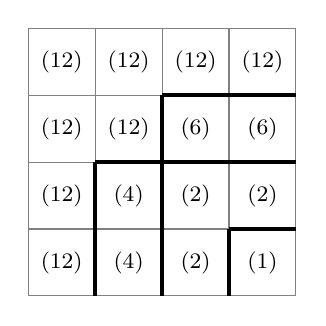
\begin{tikzpicture}[x=1cm,y=1cm,every node/.style={font=\footnotesize}]
  \draw[black!50] (0,0) grid[step=0.85] (3.4,3.4);
  \draw[line width=1.5pt]
    (1.7,2.55) -- (1.7,0)     (1.7,2.55) -- (3.4,2.55)
    (0.85,1.7) -- (3.4,1.7)   (0.85,1.7) -- (0.85,0)
    (2.55,0.85) -- (3.4,0.85) (2.55,0.85) -- (2.55,0);
  \node at (0.425,2.975) {$(12)$};
  \node at (1.275,2.975) {$(12)$};
  \node at (2.125,2.975) {$(12)$};
  \node at (2.975,2.975) {$(12)$};
  \node at (0.425,2.125) {$(12)$};
  \node at (1.275,2.125) {$(12)$};
  \node at (2.125,2.125) {$(6)$};
  \node at (2.975,2.125) {$(6)$};
  \node at (0.425,1.275) {$(12)$};
  \node at (1.275,1.275) {$(4)$};
  \node at (2.125,1.275) {$(2)$};
  \node at (2.975,1.275) {$(2)$};
  \node at (0.425,0.425) {$(12)$};
  \node at (1.275,0.425) {$(4)$};
  \node at (2.125,0.425) {$(2)$};
  \node at (2.975,0.425) {$(1)$};
\end{tikzpicture}
\caption{一张关于 $\mathbb{Z}/(12)$ 两条\trCompositionSeries{}的「\trJordan--\trHolder{}表」样本。（依原书手绘图重绘。）}%
\label{fig:jordan-holder-table}
\end{figure}

\textbf{6.5.5.}\quad 注意到：
\begin{itemize}[leftmargin=2.6em,itemsep=2pt,topsep=3pt]
\item $Z_{i,j}\subset Z_{i',j'}$，若 $i\le i'$ 且 $j\le j'$；
\item $Z_{n,j}=Y_j$，且 $Z_{i,p}=X_i$；
\item $Z_{0,j}=Z_{i,0}=0$；以及
\item $Z_{i,j}\cap Z_{i',j'}=Z_{\min(i,i'),\min(j,j')}$。
\end{itemize}

\textbf{6.5.A.（练习）}\quad （对 $i$ 作\trDescendingInduction{}）证明：$Z_{i,j}/Z_{i,j-1}$ 或者为 $0$，或者同构于单成员 $Y_j/Y_{j-1}$。

类似地，对 $Z_{i,j}/Z_{i-1,j}$ 也有类似的陈述。在这张矩形阵列中，若这两个（横向或纵向相邻的）格中之项的商非零，就在二者之间画一条\emph{粗线}，并用该单群的（\trIsomorphismClass{}）为这条线作标记（仍见图~\ref{fig:jordan-holder-array}）。

考虑该阵列中任何一个 $2\times 2$ 子方块：
\[
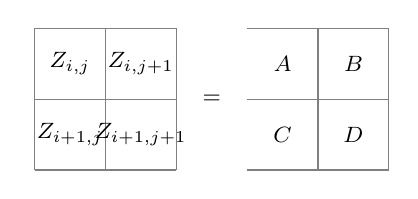
\begin{tikzpicture}[baseline={(current bounding box.center)},every node/.style={font=\footnotesize}]
  \draw[black!50] (0,0) grid[step=0.9] (1.8,1.8);
  \node at (0.45,1.35) {$Z_{i,j}$};
  \node at (1.35,1.35) {$Z_{i,j+1}$};
  \node at (0.45,0.45) {$Z_{i+1,j}$};
  \node at (1.35,0.45) {$Z_{i+1,j+1}$};
  \node at (2.25,0.9) {$=$};
  \draw[black!50] (2.7,0) grid[step=0.9] (4.5,1.8);
  \node at (3.15,1.35) {$A$};
  \node at (4.05,1.35) {$B$};
  \node at (3.15,0.45) {$C$};
  \node at (4.05,0.45) {$D$};
\end{tikzpicture}
\]
我们将看到，方块内部的诸粗线必构成如下五种花样之一（每一种都在图~\ref{fig:jordan-holder-table} 中出现过）。
\[
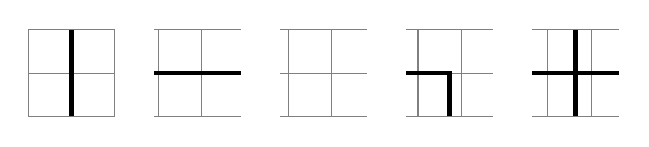
\begin{tikzpicture}[baseline={(current bounding box.center)},every node/.style={font=\footnotesize}]
  \draw[black!50] (0,0) grid[step=0.55] (1.1,1.1);
  \draw[line width=1.5pt] (0.55,0) -- (0.55,1.1);
  \draw[black!50] (1.6,0) grid[step=0.55] (2.7,1.1);
  \draw[line width=1.5pt] (1.6,0.55) -- (2.7,0.55);
  \draw[black!50] (3.2,0) grid[step=0.55] (4.3,1.1);
  \draw[black!50] (4.8,0) grid[step=0.55] (5.9,1.1);
  \draw[line width=1.5pt] (4.8,0.55) -- (5.35,0.55) -- (5.35,0);
  \draw[black!50] (6.4,0) grid[step=0.55] (7.5,1.1);
  \draw[line width=1.5pt] (6.95,0) -- (6.95,1.1) (6.4,0.55) -- (7.5,0.55);
\end{tikzpicture}
\]
由 $A=B\cap C$ 可见：(i) 若 $D=B$，则 $A=C$；(ii) 若 $D=C$，则 $A=B$。这便处置了前三种情形。

再设 $D/B$ 与 $D/C$ \emph{都}非零（从而是单的）。若 $B=C$，我们便处于第四种（「肘形」）情形。

最后，若不然，我们将看到 $D/B\cong C/A$（类似地，$D/C\cong B/A$），于是我们便处于第五种情形。考虑映射 $C\to D/B$。那么由 $A=B\cap C$（\S6.5.5），$A$ 恰是这个映射的\trKernel。于是我们有一个\trMonomorphism{} $C/A\hookrightarrow D/B$。由 $D/B$ 的单性，要么 $C/A$ 为零，要么这个\trMonomorphism{}实际上是一个\trIsomorphism{} $C/A\overset{\sim}{\hookrightarrow}D/B$。\hfill$\square$

\textbf{6.5.B.（练习）}\quad 证明\trJordan--\trHolder{}定理。提示：注意到那些加粗的线可以解释为一些路径：从表的右缘出发、走到表的底部、途中恰拐一次左弯。这将给出一个\trBijection，把一条滤过的诸单商对应到另一条滤过的诸单商。

\textbf{6.5.C.（练习）}\quad 证明：\trFiniteLength{}对象 $M$ 的每个\trSubquotient{}都具有\trFiniteLength{}。一条可能的进路：设该\trSubquotient{}为 $M''/M'$，其中 $M'\subseteq M''\subseteq M$。为 $M$ 选定一条\trCompositionSeries{} $M_\bullet$。用类似的方式再作一张新的矩形表，这次使用\trCompositionSeries{} $M_\bullet$ 与滤过 $0\subseteq M'\subseteq M''\subseteq M$。仿照\trJordan--\trHolder{}定理之证明的进路，对路径作合适的思考。

\textbf{6.5.D.（练习）}\quad 证明：\trLength{}在\trExactSequence{}中是可加的：若 $0\to M'\to M\to M''\to 0$ 是一个\trExactSequence，则 $\ell(M)=\ell(M')+\ell(M'')$。（\emph{不要}假设这些对象都具有\trFiniteLength{}。）

\textbf{6.5.E.（练习）}\quad 证明：\trFiniteLength{}\trModule{}的任何一条滤过都能\trRefine{}成一条\trCompositionSeries{}。

\textbf{6.5.F.（不重要的练习）}\quad 证明：$\scr{C}$ 中具有\trFiniteLength{}的诸对象构成 $\scr{C}$ 的一个\trFullSubcategory。

由\trGroup{}组成的\trCategory{}并不构成一个\trAbelianCategory，故定理~6.5.1 不能直接推出群的传统\trJordan--\trHolder{}定理。不过，同一个证明无须改动即可适用，只是要多加一个输入。

\textbf{6.5.G.（我们不会用到的练习）}\quad 证明群的\trJordan--\trHolder{}定理。你将需要\trSecondIsomorphismTheorem{}（second isomorphism theorem）：若 $N_1$ 与 $N_2$ 是\trGroup{} $G$ 的两个\trNormalSubgroup{}（normal subgroups），则 $N_1N_2$ 构成 $G$ 的一个\emph{正规}子群，且 $N_2/(N_1\cap N_2)\cong(N_1N_2)/N_1$。

\textbf{6.5.6. 若干只对环上的模才特有的补充事实。}

现在我们把这些概念专门用于\trCategory{} $\catMod{A}$。

\textbf{6.5.H.（练习）}\quad 证明：$\catMod{A}$ 的单对象恰是形如 $A/\mathfrak{m}$ 的那些对象，其中 $\mathfrak{m}$ 是 $A$ 的一个\trMaximalIdeal。

\textbf{6.5.I.（练习）}\quad 设 $M$ 是一个\trFiniteLength{}的 $A$-\trModule，而 \eqref{eq:composition-series-filtration} 是 $M$ 的一条\trCompositionSeries{}，其中 $M_i/M_{i-1}\cong A/\mathfrak{m}_i$（诸 $\mathfrak{m}_i$ 是\trMaximalIdeal，未必互不相同）。证明：$M$ 被 $\mathfrak{m}_1\cdots\mathfrak{m}_n$ \trAnnihilate{}。等价地，$M$ 是一个 $A/(\mathfrak{m}_1\cdots\mathfrak{m}_n)$-\trModule。

现在设列表 $(\mathfrak{m}_1,\dots,\mathfrak{m}_n)$ 由互不相同的\trMaximalIdeal{} $\mathfrak{n}_1,\dots,\mathfrak{n}_s$ 组成，它们分别以重数 $\ell_1,\dots,\ell_s$ 出现。（这些正是定义~6.5.2 中提到的「精化」\trLength{}。）

由\trChineseRemainderTheorem，
\[
A/\mathfrak{m}_1\cdots\mathfrak{m}_n\cong A/\mathfrak{n}_1^{\ell_1}\cdots\mathfrak{n}_s^{\ell_s}\cong A/\mathfrak{n}_1^{\ell_1}\times\cdots\times A/\mathfrak{n}_s^{\ell_s}.
\]
设 $1\le i\le s$，取 $A$ 中的一个元素 $e_i$，使得 $e_i\equiv 1\pmod{\mathfrak{n}_i^{\ell_i}}$，且当 $i\neq j$ 时 $e_i\equiv 0\pmod{\mathfrak{n}_j^{\ell_j}}$。诸 $e_i$ 的存在性由\trChineseRemainderTheorem{}保证。

\textbf{6.5.J.（练习）}\quad 证明：$M\cong e_1M\times\cdots\times e_sM$，且 $e_iM$ 是一个\trFiniteLength{}的\trModule，其全部单商都是 $A/\mathfrak{n}_i$。于是 $M$ 是若干块的乘积，其中每一块都带有\trCompositionSeries{}，且\trCompositionSeries{}里只有一种类型的「单因子」。

\textbf{6.5.K.（练习）}\quad 设 $M$ 是一个\trFiniteLength{}的 $A$-\trModule。证明：$M$ 是\trFinitelyGenerated{}的，且 $\Supp M$ 由 $\Spec A$ 的有限多个点组成，并且全是\trClosedPoint。（其逆命题将在\trNoetherian{}假设下作为练习~6.6.X(a) 得到证明。）这样，我们便有了「$M$ 在这些闭点中每一点处的\trLength{}」这一观念。

\textbf{6.5.7.}\ \emph{\trhDefinition{}。}\quad 若 $A$ 作为其自身上的\trModule{}具有\trFiniteLength{}，则称 $A$ 是一个\textbf{\trArtinian{}环}（Artinian ring）。若 $A$ 进而还是一个\trLocalRing，则称 $A$ 是一个\textbf{\trArtin{}或\trArtinian{}局部环}（Artin or Artinian local ring）。

\textbf{6.5.8.}\ \emph{把这套语言用于\trScheme{}。}\quad 接下来我们考虑概形 $X$ 上的\trQCSheaf{}之\trCategory{} $\catQCo_X$。对于 $X$ 上\trFiniteLength{}的\trQCSheaf，我们有\trLength{} $\ell(\scr{F})$ 这一观念。

\textbf{6.5.L.（练习）}\quad 证明：$\catQCo_X$ 的单对象恰是那些同构于\trClosedPoint{}的\trStructureSheaf{}的对象。

\textbf{6.5.M.（练习）}\quad 设 $\scr{F}$ 是 $\catQCo_X$ 中一个具有\trFiniteLength{}的成员。证明：$\scr{F}$ 是有限型的，且 $\Supp\scr{F}$ 由 $X$ 的有限多个点组成，并且全是\trClosedPoint。（其逆命题将在\trNoetherian{}假设下作为练习~6.6.X(b) 得到证明。）请说明如何定义 $\scr{F}$ 在 $\Supp\scr{F}$ 中某一点处的\trLength{}。

\textbf{6.5.9.}\ \emph{\trhDefinition{}。}\quad 所谓\textbf{\trScheme{}的\trLength{}}（length of a scheme），就是其\trStructureSheaf{} $\OO_X$（在 $\catQCo_X$ 中）的\trLength{}。若 $\OO_X$ 具有\trFiniteLength{}，则称概形 $X$ 是\textbf{\trFiniteLength{}}的，或称其为\textbf{\trArtinian}的。


\section{概形可视化：相伴点与零因子}

模的\emph{\trAssociatedPoint}理论，是把\trSupport{}观念进一步精细化（\S4.1.7）。
\trAssociatedPoint{}将帮助我们理解并可视化\trNilpotent{}元，并把「\trRationalFunction」%
的观念推广到非\trIntegral{}的\trScheme。它们还有一些我们用不上的用途，例如经由它们
与\trPrimaryDecomposition{}（primary decomposition）的联系。而对我们来说，它们最大的用处或许在于帮助
我们理解并可视化（非）\trZerodivisor——后者将经由有效\trCartierDivisor{}与%
\trLineBundle、\trRegularSequence{}（regular sequences）、\trDepth{}与\textbf{\trCM}（Cohen--Macaulay）性等话题反复登场。

现在就来讨论\trAssociatedPoint{}并没有什么特别的理由，本节可以独立阅读，任君在闲暇时
再看。但这是一次练习几何可视化、并学一些有用代数的好机会。

\textbf{6.6.1.\ 动机。}\quad 图~\ref{fig:six-associated-points} 是某个\trScheme{} $X$ 的
一幅草图。我们看到两个\trConnectedComponent{}与三个\trIrreducibleComponent。$X$ 的诸%
\trIrreducibleComponent{}的\trDimension{}分别为 $2$、$1$ 与 $1$，尽管要等到第 12 章，
我们才能对「\trDimension」有确切的理解。两个\trConnectedComponent{}都是非\trReduced{}的。

在这幅图里还能多看出一点东西，本节将借助「\trAssociatedPoint」把它说精确。那个可约的%
\trConnectedComponent{}似乎在不同\trLocus{}上有着程度不同的非\trReduced{}行为。概形 $X$
有六个\trAssociatedPoint，它们是图中「可见」的那些\trIrreducible{}子集的\trGenericPoint。%
$X$ 上的一个函数是\trZerodivisor，只要它的\trZeroSet{}含有这六个\trIrreducible{}子簇中的
任何一个。

\begin{figure}[htbp]
\centering
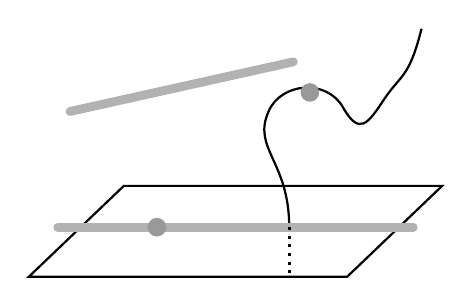
\begin{tikzpicture}[scale=1.05]
  \draw[line width=3.2pt,gray!60,line cap=round] (-2.6,1.9) -- (0.1,2.5);
  \draw[thick] (0.05,0.5) .. controls (0.05,1.3) and (-0.4,1.45) .. (-0.2,1.9)
    .. controls (-0.05,2.25) and (0.5,2.3) .. (0.7,1.95)
    .. controls (0.9,1.6) and (1.0,1.75) .. (1.2,2.05)
    .. controls (1.4,2.35) and (1.5,2.3) .. (1.65,2.9);
  \fill[gray!80] (0.3,2.13) circle (3.2pt);
  \draw[thick] (-3.1,-0.1) -- (0.75,-0.1) -- (1.9,1.0) -- (-1.95,1.0) -- cycle;
  \draw[line width=3.2pt,gray!60,line cap=round] (-2.75,0.5) -- (1.55,0.5);
  \fill[gray!80] (-1.55,0.5) circle (3.2pt);
  \draw[dotted,line width=1.1pt] (0.05,0.5) -- (0.05,-0.08);
\end{tikzpicture}
\caption{这个概形有六个\trAssociatedPoint，其中三个是\trEmbeddedPoint。一个函数只要在这
六个点中的任何一处消失，便是\trZerodivisor。（依原书手绘图重绘。）}%
\label{fig:six-associated-points}
\end{figure}

设 $M$ 是\trNoetherian{}环 $A$ 上的一个\trFinitelyGenerated{}\trModule。比如说，$M$ 也可以
就是 $A$ 自身。于是 $\Spec A$ 中有一些特殊的点，对理解 $M$ 而言尤为关键。它们就是 $M$ 的%
\emph{\trAssociatedPoint}（或者等价地说，$M$ 的\emph{\trAssociatedPrimeIdeal{}}（associated prime
ideals）——这两个术语我们将不加区分地混用）。作为动机，我们列出相伴点的亿十条性质，
把它们留给你依据本节其余部分所发展的理论去逐一验证。

在你阅读本节的过程中，不妨把
\[
M=A=k[x,y]/(y^2,\,xy)
\]
（\cref{fig:nonreduced-y2xy}）记在心头，作为贯穿本节的例子。

\textbf{6.6.2. 相伴点的亿十条性质。}\quad 下面是我们要证明的相伴点诸性质中的一部分。

相伴点只有有限多个：$\operatorname{Ass}_A M\subset\Spec A$。

$M$ 的\trSupport{}就是 $M$ 的诸\trAssociatedPoint{}的\trClosure：%
$\Supp M=\overline{\operatorname{Ass}_A M}$。$M$ 的任何一个\trSubmodule{}的\trSupport，是
$M$ 的诸\trAssociatedPoint{}中某个子集的\trClosure。$M$ 的任何一个元素的\trSupport，是
$M$ 的诸\trAssociatedPoint{}中某个子集的\trClosure。

$M$ 的诸\trAssociatedPoint，恰好就是对一切 $\mathrm{m}\in M$ 而言 $\Supp\mathrm{m}$ 的诸%
\trIrreducibleComponent{}的\trGenericPoint。$M$ 的诸\trAssociatedPoint，恰好是那些为%
\trIrreducible{}的诸 $\Supp\mathrm{m}$（$\mathrm{m}$ 跑遍 $M$ 的元素）的\trGenericPoint。%
$M$ 的\trAssociatedPrimeIdeal{}（associated primes），恰好就是那些作为 $M$ 中某个元素的\trAnnihilatorIdeal{}而出现的%
\trPrimeIdeal。

取「\trAssociatedPoint」与\trLocalization{}交换。因此这个观念本质上是几何的，这将使我们
得以（在 \S6.6.32 中）把它推广到局部诺特概形上的\trCoherentSheaf。

\trAssociatedPoint{}在正合列中的表现\emph{相当}好。例如，\trSubmodule{}的诸%
\trAssociatedPoint{}是原\trModule{}的诸\trAssociatedPoint{}的一个子集。

若 $I\subset A$ 是一个\trIdeal，则 $A/I$ 的\trAssociatedPrimeIdeal{} $\mathfrak{p}$，恰好就是那些使某个%
$\mathfrak{p}$-\trPrimary{}理想出现在 $I$ 的\trPrimaryDecomposition{}之中的 $\mathfrak{p}$。

我们将反复使用如下事实：\emph{$A$ 的一个元素是\trZerodivisor，当且仅当它在某个%
\trAssociatedPoint{}处消失}。

$A$ 的一个元素是\trNilpotent{}的，当且仅当它在每一个\trAssociatedPoint{}处消失。$\Spec A$
中使\trStalk{} $A_{\mathfrak{p}}$ 非\trReduced{}的那些点 $[\mathfrak{p}]$ 的\trLocus，是诸%
\trAssociatedPoint{}中某个子集的\trClosure。

一个处在另一个\trAssociatedPoint{}的\trClosure{}之中的\trAssociatedPoint，称为一个%
\emph{\trEmbeddedPoint}。若 $A$ 是\trReduced{}的，则 $\Spec A$ 没有\trEmbeddedPoint。%
$\mathbb{A}^n_k$ 中的\trHypersurface{}没有\trEmbeddedPoint。我们日后将看到：\trCompleteIntersection{}%
（complete intersections）没有\trEmbeddedPoint{}（\S26.2.7）。

$M$ 的元素由它们在诸\trAssociatedPoint{}处的\trLocalization{}所确定。相应的层
$\widetilde{M}$（\cref{ex:module-sheaf-on-base}）的\trSection{}由它们在诸%
\trAssociatedPoint{}处的\trGerm{}所确定。

以上讨论立即给出「局部诺特概形上的\trCoherentSheaf{}的\trAssociatedPoint」这一观念，
它带有这里描述的全部好性质。「局部诺特概形 $X$ 的\trAssociatedPoint」（不显式提及凝聚层）
一语，意思是「$\OO_X$ 的\trAssociatedPoint」；\textbf{\trEmbeddedPoint}亦同理。

我们现在就来建立这亿十条事实。

\textbf{6.6.3. 有关\trSupport{}观念的更多内容。}

$A$-\trModule{} $M$ 的\emph{\trAssociatedPoint}观念，是对\emph{\trSupport}观念的精细化
（在 $M$ 是\trNoetherian{}环 $A$ 上的\trFinitelyGenerated{}\trModule{}的情形）。（在下文
中，除非必要，我们不对 $A$ 是\trNoetherian{}的或 $M$ 是\trFinitelyGenerated{}的作任何
假设。）为作好铺垫，回忆（\S4.1.7）：$\mathrm{m}\in M$ 的\emph{\trSupport}
\[
\Supp\mathrm{m}=\{[\mathfrak{p}]\in\Spec A\ :\ \mathrm{m}_{\mathfrak{p}}\neq 0\}
\]
是一个\trClosedSubset，从而形如某个 $I$ 的 $V(I)$。练习~6.6.A 将给出「最佳的这个」$I$。
定义 $A$-\trModule{} $M$ 中元素 $\mathrm{m}$ 的\textbf{\trAnnihilatorIdeal{}}（annihilator ideal）
$\operatorname{Ann}_A\mathrm{m}\subset A$ 为：
\[
\operatorname{Ann}_A\mathrm{m}:=\{a\in A\ :\ a\mathrm{m}=0\}
  =\ker\bigl(A\xrightarrow{\times\mathrm{m}}M\bigr).
\]
当下标 $A$ 由上下文自明时，便略去不写。

\textbf{6.6.A.（轻松的重要练习）}\quad 证明：$\Supp\mathrm{m}=V(\operatorname{Ann}\mathrm{m})$。

回忆（\cref{thm:support-of-sheaf}）
\[
\Supp\widetilde{M}=\{[\mathfrak{p}]\in\Spec A\ :\ \widetilde{M}_{\mathfrak{p}}\neq 0\},
\]
以及与之类似的、\emph{\trModule{} $M$ 的\trSupport}的\cref{thm:support-of-module}：
\begin{equation*}\tag{6.6.3.1}\label{eq:supp-module-definition}
\Supp M:=\{[\mathfrak{p}]\in\Spec A\ :\ M_{\mathfrak{p}}\neq 0\},
\end{equation*}
于是 $\Supp M=\Supp\widetilde{M}$。若 $M$ 是由 $\mathrm{m}\in M$ 生成的主模（principal
module），则
\[
\Supp M=\Supp A\mathrm{m}=\Supp\mathrm{m}=V(\operatorname{Ann}\mathrm{m}).
\]

\trSupport{}与\trAssociatedPoint{}这两个观念在正合列中、以及在\trLocalization{}之下都有
良好的表现。我们现在就开始解释这一点。

\textbf{6.6.4.}\ \emph{\trSupport{}观念在正合列中表现良好。}

\textbf{6.6.B.（练习）}\quad 设 $0\to M'\to M\to M''\to 0$ 是 $A$-\trModule{}的一个%
\trShortExactSequence。

(a)~证明：$\Supp M=\Supp M'\cup\Supp M''$。

(b)~证明：若 $M$ 是\trFinitelyGenerated{}的\trModule，则 $\Supp M$ 是 $\Spec A$ 的一个%
\trClosedSubset。（提示：对生成元的个数作归纳。）

警示：一般地，$\Supp M$ 未必是闭的；考虑 $A=\mathbb{Z}$ 与
$M=\bigoplus_{\mathfrak{p}}\mathbb{Z}/(\mathfrak{p})$（对素数 $\mathfrak{p}$ 取直和）。

\textbf{6.6.C.（练习）}\quad 设 $M$ 是一个\trFinitelyGenerated{}的 $A$-\trModule，$x\in A$
在 $\Supp M$ 的所有点处取值均为 $0$，也就是说，$x$ 含于 $M$ 受支撑的每一个\trPrimeIdeal{}
之中。证明：$x$ 的某个幂 $x^n$ 零化 $M$ 的每一个元素。（提示：零化一组生成元。）

\textbf{6.6.D.（练习；将于 \S18.6 中使用）}\quad 设 $M$ 是一个\trFinitelyGenerated{}的
$A$-\trModule，$x\in A$。证明：$\Supp(M/xM)=(\Supp M)\cap V(x)$。这里 $M/xM$ 由正合列
\[
M\xrightarrow{\times x}M\longrightarrow M/xM\longrightarrow 0
\]
所定义。

\textbf{6.6.5.}\ \emph{\trhDefinition{}：\trAssociatedPoint{}与\trAssociatedPrimeIdeal{}。}

定义 $A$-\trModule{} $M$ 的\textbf{\trAssociatedPrimeIdeal{}}（associated prime ideals）为 $A$ 的形如
$\operatorname{Ann}_A(\mathrm{m})$（$\mathrm{m}\in M$）的那些\emph{\trPrimeIdeal}。定义
$M$ 的\textbf{\trAssociatedPoint}为 $\Spec A$ 中与之相应的那些点；「\trAssociatedPoint」%
与「\trAssociatedPrimeIdeal{}」这两个术语我们不加区分地混用。诸\trAssociatedPoint{}所成之集记作
$\operatorname{Ass}_A M\subset\Spec A$，下标 $A$ 在由上下文自明时省去。（为帮助记住定义
与记号，有人把它们称作 \emph{assassins}（刺客），因为它们正是那批能够毫不留情、毫无
悔意地零化\trModule{}中元素的素理想\footnote{译注：双关语——记号 $\operatorname{Ass}$
恰是「assassins」一词的后半截，而「assassinate」（行刺）又与「annihilate」（零化）音近。}。）
不过我们不会使用这个名称。

\textbf{6.6.6.}\quad 环 $A$ 的\textbf{\trAssociatedPrimeIdeal{}}（associated primes），就是把 $A$ 看作一个
$A$-\trModule{}（即取 $M=A$）时的\trAssociatedPrimeIdeal{}。

\textbf{6.6.E.（容易的练习：\trIntegralDomain{}的\trAssociatedPoint）}\quad 若 $A$ 是一个%
\trIntegralDomain，证明：$\operatorname{Ass}A=\{[(0)]\}$——零理想是唯一的\trAssociatedPrimeIdeal{}。

\textbf{6.6.F.（练习：\trHypersurface{}的\trAssociatedPoint）}\quad 给定
$f\in k[x_1,\dots,x_n]$，证明：$k[x_1,\dots,x_n]/(f)$ 的\trAssociatedPrimeIdeal{}，恰是那些由 $f$ 的素因子
生成的主理想。（你的论证将更一般地适用于任何 $f\in A$，其中 $A$ 是一个\trUFD。）

\textbf{6.6.7.}\ \emph{「$[\mathfrak{p}]\in\operatorname{Ass}_A(M)$ 当且仅当存在 $A$-%
\trModule{}的\trInclusionMap{} $A/\mathfrak{p}\hookrightarrow M$」这一观察将是必不可少
的。}下一个练习或许能把这一点敲实。

\textbf{6.6.G.（练习）}

(a)~设 $M'\subset M$。证明：$\operatorname{Ass}M'\subset\operatorname{Ass}M$。（「%
\trSupport」的相应陈述隐含在练习~6.6.B(a) 中。）

(b)~证明：$\operatorname{Ass}M\subset\Supp M$。

若 $M$ 是\trFinitelyGenerated{}的，则 $\Supp M$ 是闭的（练习~6.6.B），于是
$\overline{\operatorname{Ass}M}\subset\Supp M$。当 $A$ 是\trNoetherian{}的时，等号将在
命题~6.6.24 中证得。

\textbf{6.6.8. \trNoetherian{}环上的非零\trModule{}有\trAssociatedPoint。}

设 $\mathrm{m}$ 是 $A$-\trModule{} $M$ 的一个非零元素。注意：对 $\mathrm{m}$ 的任何非零
倍元 $x\mathrm{m}$，有 $\operatorname{Ann}\mathrm{m}\subseteq\operatorname{Ann}x\mathrm{m}%
\subsetneq A$。

\textbf{6.6.H.（练习）}\quad 设 $A$ 是\trNoetherian{}的。证明：存在某个倍元
$\mathrm{n}=x\mathrm{m}$，使得 $\mathrm{n}$ 的\emph{任何}满足 $\mathrm{yn}\neq 0$ 的非零
倍元 $y\mathrm{n}$ 都有 $\operatorname{Ann}y\mathrm{n}=\operatorname{Ann}\mathrm{n}$。

\textbf{6.6.9.\ \trhProposition。}\ ——\ \emph{沿用上一练习的记号，则
$\operatorname{Ann}\mathrm{n}$ 是一个\trPrimeIdeal。}

\emph{证明。}\ 设 $ab\in\operatorname{Ann}\mathrm{n}$，则 $ab\mathrm{n}=0$。于是要么
$b\mathrm{n}=0$（此时 $b\in\operatorname{Ann}\mathrm{n}$），要么
$a\in\operatorname{Ann}b\mathrm{n}=\operatorname{Ann}\mathrm{n}$。\hfill$\square$

于是我们便证明了下面的结论。

\textbf{6.6.10.\ \trhProposition{}（\trNoetherian{}环上的非零\trModule{}有\trAssociatedPrimeIdeal{}）。}\ ——\ %
\emph{若 $M$ 是\trNoetherian{}环 $A$ 上的一个非零\trModule，则 $\operatorname{Ass}_A M$
非空。更确切地说，对 $M$ 中任何 $\mathrm{m}\neq 0$，存在一个包含
$\operatorname{Ann}\mathrm{m}$ 的\trAssociatedPrimeIdeal{} $\mathfrak{p}$，并且对某个 $x\in A$ 有
$\mathfrak{p}=\operatorname{Ann}x\mathrm{m}$。}

\textbf{6.6.11. 在\trAssociatedPrimeIdeal{}处取\trLocalization。}

回忆一个有用的事实：$M\to\prod_{\mathfrak{p}\in\Spec A}M_{\mathfrak{p}}$ 是%
\trInjectiveMap{}（\cref{ex:module-to-product-localizations}）。我们眼下的处境还要好得多：
可以只对\emph{\trAssociatedPrimeIdeal{}}处的局部化取积。

\textbf{6.6.I.（练习）}\quad 设 $M$ 是\trNoetherian{}环 $A$ 上的一个\trModule。证明：
自然映射
\begin{equation*}\tag{6.6.11.1}\label{eq:ass-product-injection}
M\longrightarrow\prod_{\mathfrak{p}\in\operatorname{Ass}M}M_{\mathfrak{p}}
\end{equation*}
是\trInjectiveMap。提示：若\trKernel{} $K$ 非零，则 $K$ 有一个\trAssociatedPrimeIdeal{} $\mathfrak{p}$，它是
某个 $\mathrm{m}\in K\subset M$ 的\trAnnihilatorIdeal{}，而 $\mathrm{m}$ 在 $M_{\mathfrak{p}}$ 中非零。

显然，在 \eqref{eq:ass-product-injection} 中只需取诸\trAssociatedPrimeIdeal{}中的那些极大者。

\textbf{6.6.12. \trZerodivisor{}＝\trAssociatedPrimeIdeal{}的元素。}

\textbf{6.6.13.\ \trhProposition。}\ ——\ \emph{设 $f\in A$，$A$ 为\trNoetherian{}环。则
$f$ 是 $M$ 上的\trZerodivisor，当且仅当 $f$ 在 $M$ 的某个\trAssociatedPoint{}处消失。
翻译过来：\trZerodivisor{}之集是诸\trAssociatedPrimeIdeal{}的并。}

我们再一次只需诸\trAssociatedPrimeIdeal{}中的极大者。例如，若 $(A,\mathfrak{m})$ 是一个\trLocalRing，则
$\mathfrak{m}$ 是一个\trAssociatedPrimeIdeal{}，当且仅当 $\mathfrak{m}$ 的每一个元素都是\trZerodivisor。

\emph{证明。}\ 设 $f$ 在 $M$ 的某个\trAssociatedPoint{} $[\mathfrak{p}]$ 处消失。取
$\mathrm{m}$ 使 $\operatorname{Ann}\mathrm{m}=\mathfrak{p}$。则 $f\mathrm{m}=0$ 而
$\mathrm{m}\neq 0$，故 $f$ 是\trZerodivisor。

反之，若 $f$ 不在任何\trAssociatedPoint{}处消失，考虑交换图
\[
\begin{tikzcd}
M \ar[r,hook] \ar[d,"\times f"'] & \prod\limits_{\mathfrak{p}\in\operatorname{Ass}M}M_{\mathfrak{p}} \ar[d,"\times f"] \\
M \ar[r,hook] & \prod\limits_{\mathfrak{p}\in\operatorname{Ass}M}M_{\mathfrak{p}},
\end{tikzcd}
\]
其中的两行正是 \eqref{eq:ass-product-injection} 中的映射。右边的竖直箭头（乘以 $f$）由
假设是\trInjectiveMap，故左边的竖直箭头也必是\trInjectiveMap。\hfill$\square$

\textbf{6.6.14. \trAssociatedPoint{}在正合列中的表现\emph{相当}好。}

\textbf{6.6.15.\ \trhProposition。}\ ——\ \emph{设
\begin{equation*}\tag{6.6.15.1}\label{eq:ses-ass-context}
0\longrightarrow M'\longrightarrow M\longrightarrow M''\longrightarrow 0
\end{equation*}
是 $A$-\trModule{}的一个\trShortExactSequence。则
\begin{equation*}\tag{6.6.15.2}\label{eq:ass-inclusions-ses}
\operatorname{Ass}M'\subset\operatorname{Ass}M\subset\operatorname{Ass}M'\cup\operatorname{Ass}M''.
\end{equation*}}

我们来到了本节的第一个复杂证明。

\emph{证明。}\ \eqref{eq:ass-inclusions-ses} 的第一个包含关系已在练习~6.6.G(a) 中证得。

接下来设 $[\mathfrak{p}]\in\operatorname{Ass}M$，于是存在某个 $\mathrm{m}\in M$ 使
$\operatorname{Ann}\mathrm{m}=\mathfrak{p}$。我们希望找到一个\trIsomorphic{}于
$A/\mathfrak{p}$ 的、含于 $M'$ 或 $M''$ 的\trSubmodule。倘若本命题为真，我们就会期望在
「\eqref{eq:ses-ass-context} 的由 $\mathrm{m}$ 张成的那部分」中找到这样一个\trSubmodule。
于是我们转而考虑正合列
\[
0\longrightarrow A\mathrm{m}\cap M'\longrightarrow A\mathrm{m}
  \longrightarrow A\mathrm{m}/(A\mathrm{m}\cap M')\longrightarrow 0,
\]
注意这里出现的三个\trModule{}都是 \eqref{eq:ses-ass-context} 中相应\trModule{}的%
\trSubmodule。所以，由练习~6.6.G(a)，只须在这种「特殊情形」中证明本结论即可；而它可以
改写为
\[
0\longrightarrow I/\mathfrak{p}\longrightarrow A/\mathfrak{p}\longrightarrow A/I
  \longrightarrow 0,
\]
其中 $I$ 是把 $\mathrm{m}$ 视为\trModule{} $A\mathrm{m}/(A\mathrm{m}\cap M')$ 的元素时
的\trAnnihilatorIdeal{}。为方便起见，令 $B=A/\mathfrak{p}$（一个\trIntegralDomain），于是我们把这个
正合列进一步改写为下图的上行：
\[
\begin{tikzcd}
0 \ar[r] & J \ar[r] \ar[d,hook] & B \ar[r] \ar[d,hook] & B/J \ar[r] \ar[d,hook] & 0 \\
0 \ar[r] & M' \ar[r] & M \ar[r] & M'' \ar[r] & 0.
\end{tikzcd}
\]
现在把这一行 $B$-\trModule{}在 $(0)\subset B$ 处局部化，它便成为分式域 $K(B)$ 上%
\trVectorSpace{}的一个正合列，且中央元素是一维的：
\[
0\longrightarrow J\otimes K(B)\longrightarrow K(B)
  \longrightarrow(B/J)\otimes K(B)\longrightarrow 0.
\]
于是 $J\otimes K(B)$ 与 $(B/J)\otimes K(B)$ 这两端之一必有一个非零元素，它（把我们的
论证逆向追踪回去）给出 $M'$ 或 $M''$ 的一个元素，其\trAnnihilatorIdeal{}恰为 $\mathfrak{p}$。%
\hfill$\square$

\textbf{6.6.16.}\ \emph{警示性例子。}\quad $\mathbb{Z}$-\trModule{}的\trShortExactSequence
\[
0\longrightarrow\mathbb{Z}\xrightarrow{\times 2}\mathbb{Z}
  \longrightarrow\mathbb{Z}/2\longrightarrow 0
\]
（连同容易的练习~6.6.E）表明：$\operatorname{Ass}M=\operatorname{Ass}M'\cup\operatorname{Ass}M''$
并不总是成立。然而，有时我们仍能保证 $M''$ 的某些\trAssociatedPrimeIdeal{}提升为 $M$ 的\trAssociatedPrimeIdeal{}，届时将在
\S6.6.20 中看到。

\textbf{6.6.17. \trNoetherian{}环上的\trFinitelyGenerated{}\trModule{}只有有限多个%
\trAssociatedPoint{}／\trAssociatedPrimeIdeal{}。}

\textbf{6.6.J.（重要练习）}\quad 设 $M$ 是\trNoetherian{}环 $A$ 上的一个\trFinitelyGenerated{}%
\trModule。证明：$M$ 有一条（有限的）滤过（filtration）
\begin{equation*}\tag{6.6.17.1}\label{eq:filtration-quotient-primes}
0=M_0\subset M_1\subset\cdots\subset M_n=M,
\end{equation*}
其中对某个\trPrimeIdeal{} $\mathfrak{p}_i$ 有 $M_{i+1}/M_i\cong A/\mathfrak{p}_i$。
提示：借助命题~6.6.10，从左到右归纳地搭建 \eqref{eq:filtration-quotient-primes}，并证明
该过程终会终止。

\textbf{6.6.K.（练习）}\quad 设 $A$-\trModule{} $M$ 有一条有限滤过%
\eqref{eq:filtration-quotient-primes}，且不对\trFinitelyGenerated{}性或\trNoetherian{}性
作任何假设。证明：$M$ 的每一个\trAssociatedPrimeIdeal{}都作为诸 $\mathfrak{p}_i$ 之一出现。特别地，在这个
假设下（例如，若 $M$ 是\trNoetherian{}环上的\trFinitelyGenerated{}\trModule），$M$ 只有%
\emph{有限多个}\trAssociatedPoint{}／\trAssociatedPrimeIdeal{}。（提示：练习~6.6.E 与命题~6.6.15。）

\textbf{6.6.18.}\ \emph{警示：非相伴的素理想可能不可避免地出现在%
\eqref{eq:filtration-quotient-primes} 的诸商之中。}\quad 例子~6.6.16 表明，非相伴的素理想
可能出现在 \eqref{eq:filtration-quotient-primes} 的诸商之中，尽管在那样的情形里，缘由只是
滤过选得不明智。但更好的选择并不总能补救这一问题：

\textbf{6.6.L.（练习）}\quad 考虑环 $A=k[x,y]$ 上的\trModule{} $M=(x,y)\subset A$。证明：
$M$ 的\emph{任何}滤过 \eqref{eq:filtration-quotient-primes} 都含有某个商 $A/\mathfrak{p}_i$，
其中 $\mathfrak{p}_i$ \emph{不是}\trAssociatedPrimeIdeal{}。

\textbf{6.6.19.}\ \emph{\trhRemark{}。}\quad 然而，并非满盘皆输：练习~6.6.P 将证明，对
$M$ 的任何滤过 \eqref{eq:filtration-quotient-primes} 中的任何商 $A/\mathfrak{p}_i$，
$\mathfrak{p}_i$ 必\emph{包含} $M$ 的一个\trAssociatedPrimeIdeal{}。

\textbf{6.6.20. \trAssociatedPoint{}在正合列中的表现\emph{相当}好（续）。}

\textbf{6.6.21.\ \trhProposition。}\ ——\ \emph{设 $A$ 是\trNoetherian{}环。我们继续考虑
$A$-\trModule{}的\trShortExactSequence}
\[
0\longrightarrow M'\longrightarrow M\longrightarrow M''\longrightarrow 0
\]
\emph{设 $\mathfrak{p}\in\operatorname{Ass}M''$，但 $\mathfrak{p}\notin\Supp M'$（这是比
$\mathfrak{p}\notin\operatorname{Ass}M'$ 更强的假设）。则 $\mathfrak{p}\in\operatorname{Ass}M$。}

我们来到了本节的第二个复杂证明。

\emph{证明。}\ 取 $\mathrm{m}''\in M''$ 使在 $M''$ 中
$\mathfrak{p}=\operatorname{Ann}\mathrm{m}''$。取 $\mathrm{m}''\in M''$ 在 $M$ 中的一个
提升 $\mathrm{m}\in M$。我们采用与命题~6.6.15 的证明类似的策略。考虑「\trShortExactSequence{}%
的包含」：
\[
\begin{tikzcd}
0 \ar[r] & \ker(A\mathrm{m}\to A\mathrm{m}'') \ar[r] \ar[d] & A\mathrm{m} \ar[r] \ar[d] & A\mathrm{m}'' \ar[r] \ar[d] & 0 \\
0 \ar[r] & M' \ar[r] & M \ar[r] & M'' \ar[r] & 0.
\end{tikzcd}
\]
由于 $\Supp(\ker(A\mathrm{m}\to A\mathrm{m}''))\subset\Supp M'$、%
$\operatorname{Ass}(A\mathrm{m})\subset\operatorname{Ass}M$、%
$\operatorname{Ass}(A\mathrm{m}'')\subset\operatorname{Ass}M''$（练习~6.6.B(a) 与
练习~6.6.G(a)），我们已经把问题化归为考虑上行而非下行。上行可以方便地改写为
\[
0\longrightarrow\mathfrak{p}/I\longrightarrow A/I\longrightarrow A/\mathfrak{p}
  \longrightarrow 0
\]
（这里 $I=\operatorname{Ann}(\mathrm{m})$），而我们的假设翻译过来即
$[\mathfrak{p}]\notin\Supp(\mathfrak{p}/I)$。为方便起见，令 $B=A/I$，于是我们现在可以
考虑序列
\[
0\longrightarrow\mathfrak{q}\longrightarrow B\longrightarrow B/\mathfrak{q}
  \longrightarrow 0,
\]
其中 $\mathfrak{q}$ 是素的，并带有那个引人混淆的假设
$[\mathfrak{q}]\notin\Supp\mathfrak{q}$。

从这个引人混淆的假设出发，存在 $B$ 的一个元素 $b$，它在 $\Supp\mathfrak{q}$ 上消失，
却在 $[\mathfrak{q}]$ 处不消失。翻译过来：(i)~$b$ 属于 $\Supp\mathfrak{q}$ 中的所有素
理想，但 (ii)~$b\notin\mathfrak{q}$。于是由 (i)，存在 $b$ 的某个幂 $b^n$ 零化 $\mathfrak{q}$
的所有元素（练习~6.6.C，它之所以适用，是因为 $\mathfrak{q}$ 是\trFinitelyGenerated{}的，
而这又由 $A$ 的\trNoetherian{}性得到）。由 (ii)，$b^n\notin\mathfrak{q}$。

于是，$\operatorname{Ann}(b^n)$ 由 (i) 包含 $\mathfrak{q}$，又由 (ii) 不包含
$B\smallsetminus\mathfrak{q}$ 的任何元素，故 $\operatorname{Ann}(b^n)=\mathfrak{q}$。
因此 $\mathfrak{q}$ 是 $B$ 的一个\trAssociatedPrimeIdeal{}，这（把我们的论证层层解开）表明 $\mathfrak{p}$
是 $M$ 的一个\trAssociatedPrimeIdeal{}。\hfill$\square$

\textbf{6.6.22. 极小素是相伴的。}

\textbf{6.6.M.（练习：极小素（即「\trIrreducibleComponent」）是相伴的）}\quad 设 $M$ 是%
\trNoetherian{}环 $A$ 上的\trFinitelyGenerated{}\trModule，$\mathfrak{p}\subset A$ 是
对应于 $\Supp M\subset\Spec A$ 的某个\trIrreducibleComponent{}的\trPrimeIdeal。证明：
$[\mathfrak{p}]\in\operatorname{Ass}M$。提示：练习~6.6.J 与命题~6.6.21。

\textbf{6.6.23.}\ \emph{非诺特注记。}\quad 把命题~6.6.13 与练习~6.6.M 结合起来便知：若
$A$ 是\trNoetherian{}环，则任何极小素 $\mathfrak{p}$ 的任何元素都是\trZerodivisor。
这一点无须\trNoetherian{}假设也为真：设 $s\in\mathfrak{p}$；由 $\mathfrak{p}$ 的极小性，
$\mathfrak{p}A_{\mathfrak{p}}$ 是 $A_{\mathfrak{p}}$ 中唯一的\trPrimeIdeal，故 $A_{\mathfrak{p}}$
的元素 $s/1$ 是\trNilpotent{}的（因为它含于 $A_{\mathfrak{p}}$ 的一切\trPrimeIdeal{}之中，
\cref{thm:nilradical-intersection-primes}）。于是对某个 $t\in A\smallsetminus\mathfrak{p}$
有 $ts^n=0$，故 $s$ 是 $A$ 中的\trZerodivisor。我们将在练习~12.1.H 中用到它。

\textbf{6.6.24.\ \trhProposition。}\ ——\ \emph{设 $M$ 是\trNoetherian{}环 $A$ 上的一个%
\trFinitelyGenerated{}\trModule。则 $\Supp M=\overline{\operatorname{Ass}M}$。}

\emph{证明。}\ 把练习~6.6.G(b) 与练习~6.6.M 结合起来。\hfill$\square$

\textbf{6.6.N.（练习）}\quad 证明：使 $A_{\mathfrak{p}}$ 非\trReduced{}的那些点
$[\mathfrak{p}]$ 的\trLocus，就是幂零根的\trSupport{} $\Supp\mathscr{N}$。进而证明：
局部诺特概形的「既约\trLocus」是开的。

下面这条练习为「思考一个环的\trAssociatedPrimeIdeal{}的简单方式」提供了正当性。

\textbf{6.6.O.（练习）}\quad 证明：\trPrimeIdeal{} $\mathfrak{p}\subset A$ 是\trNoetherian{}%
环 $A$ 的\trAssociatedPrimeIdeal{}，当且仅当存在 $f\in A$ 使得
$\Supp f=V(\mathfrak{p})=\overline{\{[\mathfrak{p}]\}}$。

\textbf{6.6.P.（练习；应许于注记~6.6.19）}\quad 证明：对 $M$ 的滤过%
\eqref{eq:filtration-quotient-primes} 中的每个商，都有
$\Supp A/\mathfrak{p}_i=\overline{\{[\mathfrak{p}_i]\}}\subset\Supp M$，并且每个
$\mathfrak{p}_i$ 都包含一个极小素，从而包含一个\trAssociatedPrimeIdeal{}。

\textbf{6.6.25. 「\trSupport」与「\trAssociatedPoint」同\trLocalization{}交换。}

设 $S$ 是 $A$ 的一个\trMultiplicativeSubset，$\mathfrak{p}\subset A$ 是一个与 $S$ 不交的%
\trPrimeIdeal，于是（略微滥用记号）$[\mathfrak{p}]\in\Spec S^{-1}A\subset\Spec A$
（\S3.2.9）。

\textbf{6.6.Q.（练习：$\Supp$ 与局部化交换）}\quad 证明：对任何 $A$-\trModule{} $M$，
有 $\Supp_A M\cap\Spec S^{-1}A=\Supp_{S^{-1}A}S^{-1}M$。

\textbf{6.6.26.\ \trhProposition{}（$\operatorname{Ass}$ 与局部化交换）。}\ ——\ %
\emph{设 $M$ 是\trNoetherian{}环 $A$ 上的一个\trFinitelyGenerated{}\trModule。则
$\operatorname{Ass}_A M\cap\Spec S^{-1}A=\operatorname{Ass}_{S^{-1}A}S^{-1}M$。}

\emph{证明。}\ 我们先证 $\operatorname{Ass}_A M\cap\Spec S^{-1}A\subset
\operatorname{Ass}_{S^{-1}A}S^{-1}M$。若 $\mathfrak{p}\in\operatorname{Ass}_A M$，则我们有%
\trInclusionMap{} $A/\mathfrak{p}\hookrightarrow M$。用 $S$ 取局部化（它保持单射性），得
$(S^{-1}A)/(S^{-1}\mathfrak{p})\hookrightarrow S^{-1}M$。（我们是在哪里用到
$\mathfrak{p}\in\Spec S^{-1}A$ 的？）

接下来证 $\operatorname{Ass}_{S^{-1}A}S^{-1}M\subset\operatorname{Ass}_A M\cap\Spec S^{-1}A$。
设 $\mathfrak{q}:=S^{-1}\mathfrak{p}\in\operatorname{Ass}_{S^{-1}A}S^{-1}M$，于是对某个
$s\in S$ 与 $\mathrm{m}\in M$，有 $\mathfrak{q}=\operatorname{Ann}_{S^{-1}A}(\mathrm{m}/s)$。
由于 $S$ 的元素在 $S^{-1}A$ 中都是单位，故 $\mathfrak{q}=\operatorname{Ann}_{S^{-1}A}\mathrm{m}$。
由于支撑与局部化交换，$V(\mathfrak{p})$ 必是 $\Supp\mathrm{m}$ 的一个%
\trIrreducibleComponent{}（这是因为 $\Supp\mathrm{m}\cap\Spec S^{-1}A$ 包含 $[\mathfrak{q}]$，
却不包含 $[\mathfrak{q}]$ 的任何\trGenerization）。于是由练习~6.6.M，$\mathfrak{p}$ 是
$M$ 的一个\trAssociatedPrimeIdeal{}。\hfill$\square$

\hard\ \emph{不重要的注记：}\ 我们可以去掉本命题中的\trFinitelyGenerated{}假设，只须把
证明的最后一句换成下面的话：「等价地，$\mathfrak{p}$ 在 $A/\operatorname{Ann}_A\mathrm{m}$
之上是极小的。于是由练习~6.6.M，$\mathfrak{p}$ 是某个 $a\in A/\operatorname{Ann}_A\mathrm{m}$
的\trAnnihilatorIdeal{}，从而 $\mathfrak{p}$ 是 $a\mathrm{m}$ 在 $M$ 中的\trAnnihilatorIdeal{}。」

\textbf{6.6.27. \trEmbeddedPoint{}／\trEmbeddedPrime{}。}

\textbf{6.6.28.}\ \emph{\trhDefinition{}。}\quad 那些\emph{不是} $\Supp M$ 的%
\trIrreducibleComponent{}的\trGenericPoint{}的\trAssociatedPoint，称为\textbf{%
\trEmbeddedPoint}，其相应的素理想称为\textbf{\trEmbeddedPrime{}}（embedded primes）。这样叫的动机
在于它们作为\trEmbeddedPoint{}的几何化身（\S6.6.32，稍后便讲）。例如，%
图~\ref{fig:six-associated-points} 的概形有三个\trEmbeddedPoint{}（相应的环有三个\trEmbeddedPrime{}）。

\textbf{6.6.29.}\ \emph{\trhRemark{}。}\quad 练习~6.6.F 翻译过来就是：「$\mathbb{A}^n_k$
中的\trHypersurface{}没有\trEmbeddedPoint」。更一般地，若 $A$ 是一个\trUFD，则对任何
$f\in A$，$\Spec A/(f)$ 都没有\trEmbeddedPoint。朝另一个方向推广，我们将在 \S26.2.7
看到「\trCompleteIntersection{}没有\trEmbeddedPoint」。

\textbf{6.6.R.（练习）}\quad 设 $A$ 是一个\trReduced{}环（即 $A$ 没有非零\trNilpotent{}元）。
证明：$\Spec A$ 没有\trEmbeddedPrime{}。（提示：若 $\mathfrak{p}=\operatorname{Ann}a$ 是一个\trEmbeddedPrime{}，
而 $\mathfrak{q}$ 是一个极小素，取 $b\in\mathfrak{p}\smallsetminus\mathfrak{q}$。由
$ab=0$，证明 $a\in\mathfrak{q}$。于是 $a$ 含于每一个极小素。证明 $a$ 在 $\Spec A$ 的
所有点处都消失，从而由\cref{thm:nilradical-intersection-primes}它是\trNilpotent{}的。）

于是，\trReduced{}环\emph{没有\trEmbeddedPrime{}}。更好的是：\emph{\trEmbeddedPrime{}所能零化的环元素只有
幂零元。}

\textbf{6.6.30.}\ \emph{\trhRemark{}。}\quad 练习~6.6.R 的逆命题不真。没有\trEmbeddedPrime{}的环仍可
有\trNilpotent{}元——见证为 $k[x]/(x^2)$。

\textbf{6.6.S.（练习）}\quad 证明：若 $\mathfrak{p}$ 是环 $A$ 的一个\trEmbeddedPrime{}，则
$A_{\mathfrak{p}}$ 非\trReduced{}。

\textbf{6.6.31. 把手弄脏：显式的代数练习。}

\textbf{6.6.T.（练习；见图~\ref{fig:nonreduced-y2xy}）}

(a)~设 $f$ 是 $\Spec k[x,y]/(y^2,xy)$ 上的一个函数，即 $f\in k[x,y]/(y^2,xy)$。证明：
$\Supp f$ 要么是空集，要么是原点，要么是整个空间。进而求出
$\Spec k[x,y]/(y^2,xy)$ 的诸\trAssociatedPoint。

(b)~显式地、亲手地证明：$f\in k[x,y]/(y^2,xy)$ 是\trZerodivisor，当且仅当
$f(0,0)=0$。

\textbf{6.6.U.（练习：绒毛图画练手）}\quad 设 $X=\Spec\mathbb{C}[x,y]/I$，且 $X$ 的诸%
\trAssociatedPoint{}为 $[(y-x^2)]$、$[(x-1,y-1)]$、$[(x-2,y-2)]$。（本题 (d) 将验证这样
的 $X$ 确实存在。）

(a)~把 $X$ 作为 $\mathbb{A}^2_{\mathbb{C}}=\Spec\mathbb{C}[x,y]$ 的一个子集勾画出来，
连绒毛一起画上。

(b)~你掌握的信息足以判断 $X$ 是否\trReduced{}吗？

(c)~你掌握的信息足以判断 $x+y-2$ 是否\trZerodivisor{}吗？$x+y-3$ 呢？$y-x^2$ 呢？

(d)~令 $I=(y-x^2)^3\cap(x-1,y-1)^{15}\cap(x-2,y-2)$。证明：$X=\Spec\mathbb{C}[x,y]/I$
满足本题的假设。（反问一句：存在「更小」的例子吗？存在「最小」的吗？）

\textbf{6.6.32. 几何式的定义。}

\textbf{6.6.V.（练习／定义）}\quad 定义\textbf{局部诺特概形上的\trCoherentSheaf{}的%
\trAssociatedPoint{}与\trEmbeddedPoint}。（想法／提示：仿射局部地做。）

\textbf{6.6.W.（练习）}\quad 设 $X$ 是一个局部诺特概形，$U\subset X$ 是一个%
\trOpenSubscheme。证明：自然映射
\begin{equation*}\tag{6.6.32.1}\label{eq:sections-ass-injection}
\Gamma(U,\OO_X)\longrightarrow\prod\limits_{\mathfrak{p}\in\operatorname{Ass}X\cap U}
  \OO_{X,\mathfrak{p}}
\end{equation*}
（对照 \eqref{eq:ass-product-injection}）是\trInjectiveMap。

\textbf{6.6.33.}\ \emph{\trSchemeTheoreticallyDense{}性（以及更一般地，「概形论的」这个形容词）。}\quad
概形 $X$ 的一个\trOpenSubscheme{} $U$ 称为\textbf{\trSchemeTheoreticallyDense{}}（scheme-theoretically
dense）的，若任何\trOpenSet{} $V$ 上的任何函数只要限制到 $U\cap V$ 上为 $0$ 就必为
$0$。这比通常（\trTopology）意义下的稠密性更强。例如，若 $X$ 是局部诺特的，你就可以用%
\trInjectiveMap{} \eqref{eq:sections-ass-injection}（取 $M=A$）证明：\trOpenSubscheme{}
$U\subset X$ \trSchemeTheoreticallyDense{}，当且仅当它包含 $X$ 的全部\trAssociatedPoint。

更一般地，形容词「\textbf{概形论的}」（scheme-theoretic）通常标志着一种理想论式的定义，
它充实并精细化了一个更朴素的集合论式的定义。例子将包括：
\begin{itemize}[leftmargin=2.6em,itemsep=2pt,topsep=3pt]
\item \trSchemeTheoreticallyDense{}（此处）；
\item 概形论相交（图~\ref{fig:scheme-theoretic-intersection}、练习~9.1.I、练习~10.4.B）；
\item 概形论支撑（定义~9.1.4）；
\item 概形论像（\S9.4.1）；
\item 概形论闭包（\S9.4.8）；
\item 概形论原像（\S10.3.1）；以及
\item 概形论纤维（定义~10.3.3）。
\end{itemize}

\textbf{6.6.34. 重访长度观念。}

\textbf{6.6.X.（练习）}

(a)~（练习~6.5.K 的诺特版逆命题）设 $A$ 是\trNoetherian{}环。证明：任何\trFinitelyGenerated{}%
\trModule，只要其\trSupport{}由 $\Spec A$ 的有限多个点组成、且这些点全是闭点，就必具有
有限长度。

(b)~（练习~6.5.M 的诺特版逆命题）设 $\scr{F}$ 是局部诺特概形 $X$ 上一个\trFiniteType{}%
\trQCSheaf，支撑在 $X$ 的有限多个点（全为闭点）上。证明：$\scr{F}$ 具有有限长度。

\textbf{6.6.Y.（练习）}

(a)~证明：每个有限长度概形（定义~6.5.9）只有有限多个点，并带\trDiscreteTopology。

(b)~若 $X$ 在 $\overline{k}$ 上局部有限型、具有有限长度 $\ell$，证明：
$\dim_{\overline{k}}\Gamma(X,\OO_X)=\ell$。

\textbf{6.6.35. 推广分式域：\trTotalFractionRing{}。}

\textbf{6.6.36.}\ \emph{\trhDefinition{}：局部诺特概形上的\trRationalFunction。}\quad
局部诺特概形上的\textbf{\trRationalFunction}（rational function），是指对某个包含全部%
\trAssociatedPoint{}的 $U$，$\Gamma(U,\OO_X)$ 在 \eqref{eq:sections-ass-injection} 中的%
\trImage{}之元素。等价地，有理函数之集是 $\OO_X(U)$ 在所有包含诸\trAssociatedPoint{}的
开集上的余极限。例如，在 $\Spec k[x,y]/(y^2,xy)$（\cref{fig:nonreduced-y2xy}）上，
$\frac{x-2}{(x-1)(x-3)}$ 是一个\trRationalFunction，而 $\frac{x-2}{x(x-1)}$ 则不是。

一个\trRationalFunction{}有一个极大的\textbf{\trDomainOfDefinition{}}（domain of definition），因为开集上
任何两个「作为\trRationalFunction」相合（即在足够小的、包含诸\trAssociatedPoint{}的开集上
相合）的真正函数（即\trStructureSheaf{}在该开集上的\trSection）必是同一个函数——这由
\eqref{eq:sections-ass-injection} 的单射性保证。若 $\mathfrak{p}$ 含于这个极大的\trDomainOfDefinition{}
之中（或者等价地，若存在某个包含 $\mathfrak{p}$ 的开集使 $f$ 在其上有定义），我们就说%
\trRationalFunction{} $f$ \textbf{在点 $\mathfrak{p}$ 处正则}。例如，在
$\Spec k[x,y]/(y^2,xy)$ 上，有理函数 $\frac{x-2}{(x-1)(x-3)}$ 的\trDomainOfDefinition{}由除 $1$、$3$
（即 $[(x-1)]$、$[(x-3)]$）之外的一切组成，并且在这两点之外正则。一个\trRationalFunction{}%
若在所有点处正则，就称它是\textbf{正则}的。（遗憾的是，「正则」是数学中被滥用得很有规律
的一个词，代数几何中尤甚。）

一个\trRationalFunction{} $f$ 的\trDomainOfDefinition{}之补集，称为 $f$ 的\textbf{\trIndeterminacyLocus{}}%
（indeterminancy locus）（这个短语我们将在 \S11.3.3 再次见到）。

有理函数构成一个环，称为 $X$ 的\textbf{\trTotalFractionRing{}}（total fraction ring）或\textbf{\trTotalQuotientRing{}}
（total quotient ring）。若 $X=\Spec A$ 是仿射的，则这个环称为 $A$ 的\textbf{全分式
（或商）环}。若 $X$ 是\trIntegral{}的，\trTotalFractionRing{}就是\trFunctionField{} $K(X)$——即%
\trGenericPoint{}处的\trStalk{}——于是这推广了我们早先关于 $K(\cdot)$ 的定义~5.2.1。

\textbf{6.6.Z.（练习）}\quad 证明：局部诺特概形上的有理函数环，是函数在所有包含诸%
\trAssociatedPoint{}的开集上的余极限：
\[
\colim_{(U\ :\ \operatorname{Ass}X\subset U)}\OO(U).
\]
稍微更好（但略有不同）的版本：证明一个\trRationalFunction{}就是如下数据：一个定义在
包含全部\trAssociatedPoint{}的开集 $U$ 上的函数 $f$；而两组这样的数据 $(U,f)$ 与
$(U',f')$ 定义同一个\trRationalFunction，当且仅当 $f|_{U\cap U'}=f'|_{U\cap U'}$
（对照 \S1.3.9）。若 $X$ 是\trReduced{}的，证明这与「它们在每个\trIrreducibleComponent{}
的某个开集上有定义」是同一回事。

\textbf{6.6.37.}\ \emph{\trhRemark{}：\trIntegral{}概形的\trAssociatedPoint。}\quad
为了使我们别处的某些议论在非诺特的情形下也有意义，我们指出：\trIntegral{}概形的%
\trAssociatedPoint{}观念工作得尽善尽美，因为它对\trIntegralDomain{}行之有效——只有%
\trGenericPoint{}是相伴的。特别地，上面关于\trIntegral{}概形 $X$ 的\trRationalFunction{}%
的定义与定义~5.2.1 相合：二者恰是\trFunctionField{} $K(X)$ 的元素。

\textbf{6.6.38.\ \extrahard{}\ 题外话：\trPrimary{}理想与\trAssociatedPrimeIdeal{}。}\quad \trPrimaryDecomposition{}（primary
decomposition）由国际象棋世界冠军 E.~Lasker 引入，而由数学世界冠军 E.~\trNoether{}%
公理化\footnote{译注：E.~Lasker（1868--1941），德国数学家、国际象棋世界冠军
（1894--1921 在位二十七年）。「数学世界冠军」云云，是 Vakil 对\trNoether{}的戏称。}。
我们用不着它，但为好奇的读者给出这个故事的开头。环中的\trIdeal{} $I\subset A$ 称为%
\textbf{\trPrimary{}}（primary）的，若 $I\neq A$，且 $xy\in I$ 蕴涵：要么 $x\in I$，要么对某个
$n>0$ 有 $y^n\in I$。此时 $\sqrt{I}$ 是素的，且称 $I$ 为 $\mathfrak{p}$-\trPrimary{}的。等价地，
若 $I\subset A$，则 $I$ 是 $\mathfrak{p}$-\trPrimary{}的，当且仅当 $A/I$ 只有一个\trAssociatedPrimeIdeal{}
$\mathfrak{p}$。若 $I$ 是\trNoetherian{}环 $A$ 的一个\trIdeal，那么 $A/I$ 的诸\trAssociatedPrimeIdeal{}
恰好就是一个\trPrimaryDecomposition{}中诸理想的根。这一重要故事的更多内容，例如可参看 [E, \S3.3]。


\section{\extrahard\ 非诺特环上的凝聚模}

本节是为这样两种人写的：可能要同非\trNoetherian{}环打交道的人，或者以别的方式想在更一般的背景下理解\trCoherentSheaf{}的人。即便是这些人，也应当等到很久之后再读它。除非你真的想读，否则别读！

设 $A$ 是一个\trRing。回忆一个 $A$-\trModule{} $M$ 何时称为\trFinitelyGenerated{}的、\trFinitelyPresented{}的与\trCoh{}的（\S6.4）。我们喜欢凝聚性的理由是：\trCoh{}\trModule{}构成一个\trAbelianCategory。下面是一些不难入手的练习，把这些概念为何表现良好亲手算清。其中有些重复了先前的讨论，为的是让本节内容自足。

一个\trModule{}的凝聚性这一概念，只有在环于自身之上\trCoh{}的场合才有意思。类似地，概形 $X$ 上的\trCoherentSheaf{}也只有在 $\OO_X$ \trCoh{}（「在自身之上」）时才有意思。在这种情形，凝聚性显然就与有限表现是同一回事。非\trNoetherian{}凝聚性出场的一个例子，是「\trRestrictedPowerSeries{}」（restricted power series）环 $R\langle x_1,\dots,x_n\rangle$，其中 $R$ 是带非离散赋值的 $K$（例如 $\mathbb{Q}_p$ 的\trAlgebraicClosure{}的一个完备化）的\trValuationRing{}。这与\trTate{}的 $K$ 上\trNonArchimedean{}解析几何理论有关（例如可在 [BCDKT] 中读到）。结构层凝聚性的重要性，凸显了复几何中\trOka{}定理（陈述见 \S6.4.8）的重要性。

\textbf{6.7.A.（练习）}\quad 证明：\trCoh{}蕴涵\trFinitelyPresented，而后者又蕴涵\trFinitelyGenerated。（这在 \S6.4 开头讨论过。）

\textbf{6.7.B.（练习）}\quad 证明：$0$ 是\trCoh{}的。

对练习~6.7.C--6.7.I，设
\begin{equation*}\tag{6.7.0.1}\label{eq:coherent-exercise-sequence}
0\longrightarrow M\longrightarrow N\longrightarrow P\longrightarrow 0
\end{equation*}
是 $A$-\trModule{}的一个\trExactSequence。在这一系列练习中，我们将证明：$\{M,N,P\}$ 中若有两个是\trCoh{}的，则第三个亦然——这将会大有用处。

\textbf{6.7.1.（提示）}\quad 下面的提示适用于其中好几道练习：试着写出
\[
\begin{tikzcd}[row sep=2.6em, column sep=2.8em]
0 \ar[r] & A^{\oplus p} \ar[r] \ar[d] & A^{\oplus(p+q)} \ar[r] \ar[d] & A^{\oplus q} \ar[r] \ar[d] & 0 \\
0 \ar[r] & M \ar[r] & N \ar[r] & P \ar[r] & 0{,}
\end{tikzcd}
\]
并可能用上蛇形引理~1.6.5。

\textbf{6.7.C.（练习）}\quad 证明：$N$ \trFinitelyGenerated{}蕴涵 $P$ \trFinitelyGenerated。（你只需要 \eqref{eq:coherent-exercise-sequence} 的\trRightExact{}性。）

\textbf{6.7.D.（练习）}\quad 证明：$M$、$P$ 都\trFinitelyGenerated{}蕴涵 $N$ \trFinitelyGenerated。可能的提示：\S6.7.1。（你只需要 \eqref{eq:coherent-exercise-sequence} 的\trRightExact{}性。）

\textbf{6.7.E.（练习）}\quad 证明：$N$、$P$ 都\trFinitelyGenerated{}并不必然蕴涵 $M$ \trFinitelyGenerated。（提示：若 $I$ 是一个\trIdeal，则有 $0\to I\to A\to A/I\to 0$。）

\textbf{6.7.F.（练习）}\quad 证明：$N$ \trCoh、$M$ \trFinitelyGenerated，蕴涵 $M$ \trCoh。（你只需要 \eqref{eq:coherent-exercise-sequence} 的\trLeftExactness。）

\textbf{6.7.G.（练习）}\quad 证明：$N$、$P$ 都\trCoh{}蕴涵 $M$ \trCoh。凝聚性定义（\S6.4.1）中 (i) 的提示：
\[
\begin{tikzcd}[row sep=2.2em, column sep=2.8em]
 & A^{\oplus q} \ar[dd] \ar[dr] & & \\
 & & A^{\oplus p} \ar[d] \ar[dr] & \\
0 \ar[r] & M \ar[r] \ar[d] & N \ar[r] \ar[d] & P \ar[r] \ar[dr] & 0 \\
 & 0 & 0 & & 0.
\end{tikzcd}
\]
（你只需要 \eqref{eq:coherent-exercise-sequence} 的\trLeftExactness。）

\textbf{6.7.H.（练习）}\quad 证明：$M$ \trFinitelyGenerated{}且 $N$ \trCoh{}蕴涵 $P$ \trCoh。凝聚性定义（\S6.4.1）中 (ii) 的提示：\S6.7.1。

\textbf{6.7.I.（练习）}\quad 证明：$M$、$P$ 都\trCoh{}蕴涵 $N$ \trCoh。（提示：\S6.7.1。）

\textbf{6.7.J.（练习）}\quad 证明：\trCoh{}\trModule{}的有限\trDirectSum{}是\trCoh{}的。

\textbf{6.7.K.（练习）}\quad 设 $M$ \trFinitelyGenerated{}而 $N$ \trCoh。若 $\phi\colon M\to N$ 是任意一个映射，证明：$\operatorname{Im}\phi$ 是\trCoh{}的。

\textbf{6.7.L.（练习）}\quad 证明：\trCoh{}\trModule{}之间映射的\trKernel{}与\trCokernel{}都是\trCoh{}的。

至此，我们已验证：\trCoh{}的 $A$-\trModule{}构成 $A$-\trModule{}的\trCategory{}的一个\trAbelian\trSubcategory。（必须检验的事项：$0$ 应属于此集合；它应对有限和封闭；并且它应对取\trKernel{}与\trCokernel{}封闭。）

\textbf{6.7.M.（练习）}\quad 设 $M$ 与 $N$ 是\trCoh{}\trModule{} $P$ 的两个\trCoh{}\trSubmodule。证明：$M+N$ 与 $M\cap N$ 都是\trCoh{}的。（提示：考虑那个「对的」映射 $M\oplus N\to P$。）

\textbf{6.7.N.（练习）}\quad 证明：若 $A$ 是\trCoh{}的（作为 $A$-\trModule），则\trFinitelyPresented{}\trModule{}都是\trCoh{}的。（当然，若\trFinitelyPresented{}\trModule{}都\trCoh，则 $A$ 必\trCoh，因为 $A$ 就是\trFinitelyPresented{}的！）

\textbf{6.7.O.（练习）}\quad 若 $M$ 是\trFinitelyPresented{}的且 $N$ 是\trCoh{}的，证明：$\Hom(M,N)$ 是\trCoh{}的。（提示：$\Hom$ 对第一个变量是\trLeftExact{}的。）

\textbf{6.7.P.（练习）}\quad 若 $M$ 是\trFinitelyPresented{}的，而 $N$ 是\trCoh{}的，证明：$M\otimes_A N$ 是\trCoh{}的。

